\documentclass[oneside]{ZJUthesis}

% 该文档中首字符为“%”的均为注释行,不会在论文中出现
% 论文默认为双面模式,需单面模式请将第一行换为如下所示:
% \documentclass[oneside]{ZJUthesis}
% \documentclass[twoside]{ZJUthesis}

% 取消目录中链接的颜色,方便打印
% 如需颜色,请将“false”改为“true”
\hypersetup{colorlinks=false}

% 这里几行代码使得目录中的“第几章” 和后面的章节名称不致发生重叠
\makeatletter
\renewcommand{\numberline}[1]{%
\settowidth\@tempdimb{#1\hspace{0.5em}}%
\ifdim\@tempdima<\@tempdimb%
  \@tempdima=\@tempdimb%
\fi%
\hb@xt@\@tempdima{\@cftbsnum #1\@cftasnum\hfil}\@cftasnumb}
\makeatother

%\usepackage[sectionbib]{chapterbib}
\usepackage{enumerate}
%\usepackage[linesnumbered,boxed]{algorithm2e}


\makeatletter
\def\@chapter[#1]#2{\ifnum \c@secnumdepth >\m@ne
  \if@mainmatter
    \refstepcounter{chapter}%
    \typeout{\@chapapp\space\thechapter.}%
    \addcontentsline{toc}{chapter}%
    {\protect\numberline{第 \chaptername 章}\hspace{1em}#1}
%    {\protect\numberline{\chaptername}\hspace{4em}#1}
  \else
    \addcontentsline{toc}{chapter}{#1}%
  \fi
  \else
  \addcontentsline{toc}{chapter}{#1}%
  \fi
  \chaptermark{#1}%
  \if@twocolumn
  \@topnewpage[\@makechapterhead{#2}]%
  \else
  \@makechapterhead{#2}%
\@afterheading
\fi}
\makeatother

\begin{document}
%%%%%%%%%%%%%%%%%%%%%%%%%%%%%
%% 正文字体设定
%%%%%%%%%%%%%%%%%%%%%%%%%%%%%
\songti

%%%%%%%%%%%%%%%%%%%%%%%%%%%%%
%% 论文封面部分
%%%%%%%%%%%%%%%%%%%%%%%%%%%%%
% 中文封面内容

% 中图分类号
\classification{TM391}

% 单位代码
\serialnumber{10335}

% 密级,如需密级则将其前“%”去掉
\SecretLevel{绝密}
%\SecretLevel{公开}

% 学号
\PersonalID{21221234}

\title{论文题目第一行}
% 如果标题一行写不下,就写成两行,在下面的命令里写第二行,不需要两行则注释掉
\titletl{论文题目第二行}
%\titletl{test}

%英文题目
\Etitle{English Title The 1st Line}
% 如果一行写不下,同中文题目设定,一行写不下则写两行,不需要就注释掉
\Etitletl{English Title The 2nd Line}
%\Etitletll{}

% 作者
\author{author}
\Eauthor{Author}

%\author{张睿卿}
%\Eauthor{Author}

\degree{硕士}
\Edegree{Master of Engineering}

% 导师
%\supervisor{潘纲教授}
%\Esupervisor{Prof. GangPan}
\supervisor{}
\Esupervisor{}

% 合作导师,如果有的话,去掉注释
% \cpsupervisor{}
% \Ecpsupervisor{}

% 专业名称
\major{计算机科学与技术}
\Emajor{Computer Science and Technology}

% 研究方向
\researchdm{脑机接口}
\Eresearchdm{Brain Machine Interface}

% 所属学院
\institute{计算机科学与技术学院}
\Einstitute{College of Computer Science and Technology}

%论文提交日期
\submitdate{二〇一五年四月三十日}
\Esubmitdate{2015-05-05}

% 答辨日期
\defenddate{2015-05-15}

% 生成封面
\makeCoverPage

% 生成英文封面
\makeECoverPage

%%%%%%%%%%%%%%%%%%%%%%%%%%%%%%
%% 中文题名页内容
%%%%%%%%%%%%%%%%%%%%%%%%%%%%%%
% 论文评阅人信息 注意两字名与三字名,两字职称与三字职称的写法,便于对齐
% 多余的名额直接注释掉即可,比如三个评阅人,把评阅人D,E注释掉即可
\reviewersA{评阅人\hspace{1.5em}教授\hspace{1.5em}浙江大学\hspace{1em}}
\reviewersB{评阅人\hspace{1.5em}教授\hspace{1.5em}浙江大学\hspace{1em}}
\reviewersC{评阅人\hspace{1.5em}教授\hspace{1.5em}浙江大学\hspace{1em}}
\reviewersD{评阅人\hspace{1.5em}教授\hspace{1.5em}浙江大学\hspace{1em}}
\reviewersE{评阅人\hspace{1.5em}教授\hspace{1.5em}浙江大学\hspace{1em}}

% 答辩委员会信息,如果某一个单位比较长,
% 请在其它较短后面补上{hspace{Xem}},X是比最长的单位名少几个字
% 如果实际人数少于6人,多余的注释掉即可
\chairman{委\quad 员\quad 教授\quad 浙江大学\hspace{1em}}
\commissionerA{委\quad 员\quad 教授\quad 浙江大学\hspace{1em}}
\commissionerB{委\quad 员\quad 教授\quad 浙江大学\hspace{1em}}
\commissionerC{委\quad 员\quad 教授\quad 浙江大学\hspace{1em}}
\commissionerD{委\quad 员\quad 教授\quad 浙江大学\hspace{1em}}
\commissionerE{委\quad 员\quad 教授\quad 浙江大学\hspace{1em}}

% 生成中文题名页
\maketitle


%%%%%%%%%%%%%%%%%%%%%%%%%%%%%%
%% 英文题名内容
%%%%%%%%%%%%%%%%%%%%%%%%%%%%%%
\englishtitle{English Title The 1st Line}
% 如果题名一行写不下,就写到第二行,不需要则将其注释掉
\englishtitletl{English Title The 2nd Line}
%\englishtitletll{}

% 评阅人信息,名字,职称,单位尽量用简写,否则会写不下
\EreviewersA{Name\hspace{1.5em}Professional Title\hspace{1.5em}Organization}
\EreviewersB{Name\hspace{1.5em}Professional Title\hspace{1.5em}Organization}
\EreviewersC{Name\hspace{1.5em}Professional Title\hspace{1.5em}Organization}
\EreviewersD{Name\hspace{1.5em}Professional Title\hspace{1.5em}Organization}
\EreviewersE{Name\hspace{1.5em}Professional Title\hspace{1.5em}Organization}

% 答辩委员会信息,同样尽量用简写,否则会写不下
\Echairman{Name\hspace{1.5em}Professional Title\hspace{1.5em}Organization}
\EcommissionerA{Name\hspace{1.5em}Professional Title\hspace{1.5em}Organization}
\EcommissionerB{Name\hspace{1.5em}Professional Title\hspace{1.5em}Organization}
\EcommissionerC{Name\hspace{1.5em}Professional Title\hspace{1.5em}Organization}
\EcommissionerD{Name\hspace{1.5em}Professional Title\hspace{1.5em}Organization}
\EcommissionerE{Name\hspace{1.5em}Professional Title\hspace{1.5em}Organization}

% 生成英文题名页
\makeenglishtitle


%%%%%%%%%%%%%%%%%%%%%%%%%%%%%%
%% 原创声明与版权协议页
%%%%%%%%%%%%%%%%%%%%%%%%%%%%%%

\SignautreDateA{2015}{3}{10}
\SignautreDateB{2015}{3}{10}
\SignautreDateC{2015}{3}{10}
% 生成原创声明与版权协议页
\makeOSandCPRTpage


%%%%%%%%%%%%%%%%%%%%%%%%%%%%%%
%% 论文部分开始
%%%%%%%%%%%%%%%%%%%%%%%%%%%%%%
\ZJUfrontmatter

%%%%%%%%%%%%%%%%%%%%%%%%%%%%%%
%% 勘误页,一般没有
%%%%%%%%%%%%%%%%%%%%%%%%%%%%%%
%\begin{corrigenda}
这是一个勘误\index{勘误}章节,一般情况下是没有的。
\end{corrigenda}



%%%%%%%%%%%%%%%%%%%%%%%%%%%%%%
%% 序言页,一般没有
%%%%%%%%%%%%%%%%%%%%%%%%%%%%%%
%\begin{preface}
上一版发布于2011年10月26日,发布之后的近两年来,陆陆续续收到一些邮件问关于使用中的一些问题,
我也算基本上做到一一解答。
同进也在着手准备根据提到的问题对这一版模版进行一定的修订,增补一些使用中普遍关心的难点问题。
因为事务冗杂缠身,加上关于参考文献格式调整部分的内容一直没有时间看明白,这个事情就一直拖下来了。
直到前一段断断续续看完了参考文献格式整理部分的帮助资料,搞清楚了它的实现思路原理,
才算又着手修订这一版教程。

在这过去的一年多里,接触到了\XeTeX{},对其强大的直接调用系统字体的能力表示赞叹,
于是将这个模版切换到了\XeTeX{}的环境下,将文件代码换成了对多语言兼容更好的UTF-8代码,
但同时保留对GBK码的兼容,具体不同之处会在后面的章节中提到。
因此新的一版分为UTF-8和GBK两个版本进行发布,两个版本使用上只有很细微的区别,
一般使用过程中可以忽略这个差别。

以下是原来的序言,此处照旧附上。


很早就听说过\LaTeX\index{\LaTeX}了,但却一直没有真正学习过,直到今年,需要处理一些大文档,想起了\LaTeX{}。
重新翻出\LaTeX{}的文档,从CCT开始,至于为什么是CCT,
因为Ctex\index{CTeX}提供的那个CTeX FAQ里对中文的第一个例子,就是以CCT
为例写的。
CCT是中科院的张林波研究员写的,帮助文档都是中文,看起来比较容易,但毕竟是好几年前的版本了,
更新也并不是那么及时,而且CCT\index{CCT}早期版本的字体是点阵字体,边缘很粗糙,
虽然不影响打印,但在这个年代还在用着这样的字体,着实不是那么舒服。
我又开始了第二个例子,CJK的尝试,在尝试CJK\index{CJK}的过程中,
无意中看到了CTeX的ctexart,ctexbook和ctexrep这几个基本模版,这才找到CTeX的门,
筒子们不要笑我绕了这么一大圈才摸进了CTeX的门,虽然从开始就使用的是CTeX的发行版。

这里也要说一下,CTeX提供的部分帮助文档内容也比较老了,一些操作现在新的软件虽然仍然兼容,
但已经不是新版软件推荐的做法了,比如,CTeX FAQ里面对于pdf文件的生成,
依然是先由latex.exe生成dvi文件,再由dvi文件生成ps文件,最后再生成pdf文件。
实际上,现在流行的新版\TeX{}类软件都已经将pdfTeX\index{pdfTeX}作为默认引擎,支持直接生成pdf文件,
而且dvi、ps文件的打开速度比pdf反而要慢许多。我使用的是64位系统,CTeX提供的安装包只支持32位系统,
我单独安装的MikTeX\index{MikTeX} x64\index{x64}版使用CTeX模版生成的dvi文件使用dvips\index{dvips}处理时会找不到字体,
因为这个问题,我找了很久,最后的结论是:dvips可以放弃了,直接使用dvipdfm\index{dvipdfm}更合适。

后来几天在\LaTeX{}的实践中看不少相关细节,开始对其模版产生了兴趣,
在88上\TeX{}版把置顶的ZJUthesis下了下来,就是写这个模版的基础,数学系模版。
下下来后发现这个模板给的例子pdf与当前学校使用的2008年论文模版差别老大了,从封面到目录,
章节格式,都是完全不一样,因此,决定着手做一个与学样提供的Word模版比较接近的模版。

在以2006年数学系模版为基础进行新模版编写的过程中,学了不少方法,
也发现老模版不少过时或者不合适的地方。
第一个学到的就是,从模版一开头就发现这个模版是以ctexbook这个模版为基础制作的,
做到模版完成的时候,
发现88的\TeX{}版置顶模版已经更新,我以为我白做了,
下下来一看,原来这个新的模版不是以ctexbook为基础制作的,而是更基础的\LaTeXe\index{\LaTeX}
对比自己基本完工的模版,才发现ctexbook为我省了很多工作量。只是一些修修改改就做到了很接近学校
word模版的效果。
ctexbook的新版已经直接将hyperref包打了进去,2006年数学系模版对hyperref\index{hyperref}的引用判断部分已经明显示过时,在用新版MikTeX运行的时候直接报错了。
在编写封面的时候,发现2006年的模版用了一个五列的表格,可这部分的内容只需要两列就够了,
直到我某天下载了中科院的模版后才明白,2006年版模版是从中科院模版改编而来,
中科院模版在封面上名字等内容的排列方式需要采用五列表格。这一部分,我也将其重新编写。

随着时代的推进,\LaTeX{}的各种功能包日渐丰富,很多过去只能从\LaTeXe{}代码写的功能,
如今可以通过相应的功能包直接实现,在这个模版中,我使用了几个新的功能包,
其中最新的当属刚刚发布的hyperref更新包,增加了hidelinks命令,可以直接将链接的边框去掉,
不用采用将边框颜色设为白色的方式了。

就像\LaTeX{}的版本总是在接近$\pi$的值一样,这份模版并不是完美的,比如对数学系的定理体系支持不足,
留在以后版本再发布或者请有兴趣的爱好者共同修改。编写这一版本的基本目的是没有任何\LaTeX{}基础的同学可以比较轻松地利用它给自己的毕业论文排一个满意的版面,整个模版没有留太多选项,
可供修改的选项只有两个:单面双面的选择和链接的颜色的有无。在模版中,我对绝大多数的语句,
都做了中文注释,解释其作用,方便有兴趣的同学研究,我也是一个初学者,作出的这份模版,
我想,应该是比较适合初学者胃口的。

\end{preface}


%%%%%%%%%%%%%%%%%%%%%%%%%%%%%%
%% 摘要
%%%%%%%%%%%%%%%%%%%%%%%%%%%%%%
\begin{abstract}

多年来人们在生物学医学领域的研究发现, 生物脑电活动可以通过一个非肌肉通路向外设传递信息, 这个外设被称作脑机接口。 脑机接口可以代替受损的神经系统,通过大脑信号采集,信号处理,解码为计算机指令,反馈这四步,为残障人士提供自动化服务。本论文主要研究侵入式脑电信号处理,压缩,以及EEG信号中的P300波形检测。

侵入式脑机接口在神经手术中直接植入大脑灰质, 其采集的信号具有高分辨率, 高采样率的性质,因此压缩对于信号存储和传输都是必不可少的环节。 在压缩方面,过去的神经信号压缩工作主要关注于非侵入式脑电信号,这些方法都应用了相关信号的特性。 但这些信号同侵入式信号有很大差异,所以其压缩方法不能直接套用在侵入式脑电信号中。 另一方面, 低分辨率的非侵入式脑机接口采样方便, 如脑电图(EEG)在大脑头皮非侵入式地记录神经元内离子电流产生的电位波动\cite{nie2005ele}, 所采集的信号在神经解码中广泛应用。 P300波形是大脑在决策时产生的事件相关电位中的正向偏移, 表示年轻成年人对简单的感官可分辨目标响应峰值延时约300ms。 

本文的主要工作如下:
\begin{enumerate}
\item 通过侵入式电极研究大脑运动皮层信号性质, 利用信道内部神经信号特性建立了一个完整的高保真运动皮层信号压缩框架。 该框架称为双阶编码方法, 创新地采用幅值滤波器对侵入式脑电信号的频域数据进行分割, 提出符号编码和混合编码方法分别对分割后数据进行压缩。 混合编码方法由哈弗曼编码和零长编码组合, 我们根据零分量占比分布提出了界限下降算法来求取两种编码方法的分界点。 在实验中, 我们将双阶编码方法与传统压缩方法和典型时序信号压缩方法进行了比较, 双阶编码方法可以在相同压缩率下达到更高的信号保真度, 在18\%的压缩比下达到36db的信噪比, 并保留了92\%的动作电位信号。

\item 采用深度学习的方法进行P300波形信号处理与检测。 文中, 我们分别建立了ConvP300Net和LSTMP300Net对EEG信号建模。 ConvP300Net中提出用一个6层卷积神经网络, 用局部连接层在空间维度对数据进行非共享卷积, 用卷积层对信号在时间维度进行共享卷积 , 用全连接层增强网络表达能力, 最后采用带权损失函数度量网络分类能力。 LSTMP300Net中采用一个5层网络, 其中3个中间层分别为长短时间记忆(LSTM)层。 不同于属于前向网络的卷积神经网络, LSTM层内各节点相互连接, 可以充分结合EEG信号在时间和空间维度的特性提高检测准确性,完善模型。 我们对ConvP300Net和LSTMP300Net分别用backpropagation和backpropagation through time方法进行训练, 并与相关工作进行比较, 结果ConvP300Net和LSTMP300Net在BCI竞赛数据集上分别达到80.09\%和84.47\%的识别率, 均超过已有工作对P300波形的检测效果。

\end{enumerate}





\keywords{脑机接口,压缩,卷积神经网络,长短期记忆方法,循环神经网络}
\end{abstract}

%{\pagestyle{empty}\mbox{}\newpage\pagestyle{empty}}  % 无页眉页脚的空白页
%%%%%%%%%%%%%%%%%%%%%%%%%%%%%%
%% 英文摘要
%%%%%%%%%%%%%%%%%%%%%%%%%%%%%%
\begin{englishabstract}
Brain Machine Interface (BMI) is an interface that connect neurons of brain and devices to communicate and control. BMI can substitute impaired neural system, provide automatic service to disabled people through four steps: sampling signal from brain, signal processing, signal decoding to computer instruction, and feedback. This thesis focus on invasive electroneurographic signal processing, compression and P300 wavelet detection in Electroencephalograph signal. 

Invasive electroneurographic signal with high sampling rate and multiple channel can represent high-resolution information. However, the huge quantity of data makes compression indispensable. 
In the aspect of signal compression, some related work focus on non-invasive electroneurographic signal. These methods take the consideration of signal characteristics. However, power centralizes in low frequency for non-invasive neural signal, therefore signal can be compressed through low pass filter directly. But the high frequency part of invasive BCI includes action potential (spike), which can be decoded effectively. As a consequence, traditional compression methods cannot be directly used in invasive BCI. In this thesis, we explore the characteristics of electroneurographic signal from motor cortex and provide a high fidelity compression framework for it. 

On the other hand, non-invasive BMI provides low-resolution data easily, like Electroencephalograph, which is popular in  neural signal decoding. As a pre task of machine execution, neural signal decoding is the core of BCI. Here we process and detect P300 wave, which is a prework of EEG signal decoding. In this thesis, we apply deep learning method to P300 wavelet detection, build convolutional neural network and recurrent neural network for EEG signal, and boost detection accuracy from both temporal and spatial dimension.



\englishkeywords{Brain Machine Interface, compression, Convolutional neural network, Long Short Term Memory, Recurrent Neural Network}

\end{englishabstract}

%{\pagestyle{empty}\mbox{}\newpage\pagestyle{empty}}  % 无页眉页脚的空白页

%%%%%%%%%%%%%%%%%%%%%%%%%%%%%%
%% 论文部分开始2
%%%%%%%%%%%%%%%%%%%%%%%%%%%%%%
\ZJUfrontmatterTwo

%%%%%%%%%%%%%%%%%%%%%%%%%%%%%%
%% 目录页
%%%%%%%%%%%%%%%%%%%%%%%%%%%%%% 
\ZJUcontents

%%%%%%%%%%%%%%%%%%%%%%%%%%%%%%
%% 插图列表
%%%%%%%%%%%%%%%%%%%%%%%%%%%%%%
\ZJUListofFigures

%%%%%%%%%%%%%%%%%%%%%%%%%%%%%%
%% 表格列表
%%%%%%%%%%%%%%%%%%%%%%%%%%%%%%
\ZJUListofTables

%%%%%%%%%%%%%%%%%%%%%%%%%%%%%%
%% 缩写、符号清单、术语表
%%%%%%%%%%%%%%%%%%%%%%%%%%%%%%
%\begin{ListofSymbol}
缩写、符号清单、术语表
\end{ListofSymbol}


%%%%%%%%%%%%%%%%%%%%%%%%%%%%%%
%% 正文内容部分开始
%%%%%%%%%%%%%%%%%%%%%%%%%%%%%%
\ZJUmainmatter

\chapter{脑机接口及相关信号}

\section{脑机接口简介}

由于现代计算机技术和神经科学学科的迅速发展,人们已经可以将大脑中的运动与计算机设备相关联,通过机器捕捉大脑中神经元的活动\cite{wolpaw2002brain}。这种为大脑和外部设备之间建立通路的方法与应用统称为脑机接口(brain computer interface,或BCI)\cite{van2009brain,donoghue2002connecting},以探索大脑活动与特定神经状态的关系。 脑机接口可以通过测量脑信号从而理解主体意愿, 而无需做出任何动作指示\cite{kostov2000parallel,allison2007brain,birbaumer2007brain}。 因此BCI对残障人士或运动皮层受损, 不能很好地与肌肉通信的病人有很大辅助作用。 比如对于脊侧索硬化\cite{allison2007brain}病人, 如果可以有效地对脑信号解码, 分析其意愿, 就可以通过外设完成相应操作, 从而辅助病人。 

现在有很多测量脑信号的技术,如fMRI (functional magnetic resonance imaging,功能性磁共振成像),NIRS(near-infrared spectroscopy,近红外光谱学),EEG(Electroencephalograph,脑电图),MEG(Magnetoencephalography,脑磁图)等。 针对不同的采集信号,其信号预处理方法也各不相同。但是BCI最基本的任务都是正确地识别次级类别并翻译成机器指令以完成用户的意愿。 脑机接口整个过程技术如图\ref{Fig:bci_brief}所示\cite{farwell1988talking},一个BCI需要包括:

\begin{enumerate}
\item{记录大脑活动}\\
	第一步, 需要用放大器采集脑信号。 
\item{提取并处理脑信号}\\
	第二步, 需要将脑信号进行预处理, 并分析其属于哪一类刺激, 即进行信号解码。 该步骤的解码部分非常重要, 包括脑信号特征提取并翻译的过程。 如果解码错误, 后面的两步就会变得无意义了。
\item{将脑信号翻译成计算机指令}\\
	第三步, 将解码后的信号发送到外部设备, 执行相关指令。
\item{最后返回给用户}\\
	最后, 外部设备将结果返回给用户。
\end{enumerate}

图\ref{Fig:bci_brief}中, 签名表示大脑神经信号的特定状态。 

\begin{figure}[htb]
\centering
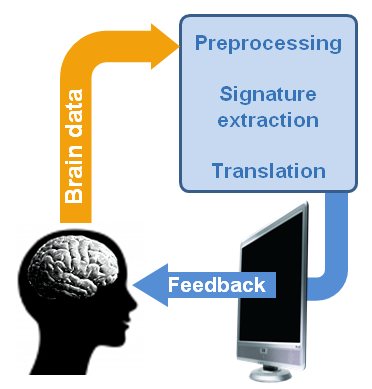
\includegraphics[scale=0.8]{Pictures/Chap1/bci_cycle_v2-2.png}
\caption{BCI 框架\cite{farwell1988talking}}
\label{Fig:bci_brief}
\end{figure}

在第二步的解码中, 采用一个信号分类器, 对不同刺激产生的信号进行分类。 已有很多方法针对信号解码提出一些的模式识别方法。 大多数有效方法基于机器学习模型\cite{blankertz2006berlin,lotte2007review,muller2008machine}, 如支持向量机(SVM)\cite{cortes1995support}, 隐马尔科夫模型(HMM)和神经网络模型都曾被用于神经解码。 此外, W.Wu等人基于卡尔曼滤波器建立了一个实时解码系统, 对运动皮层手臂区域大约40个神经元上所采集到的spike活动进行解码, 并证明其效果好于之前用到的线性滤波器技术\cite{wu2003neural}。 在根据神经信号进行手臂路径跟踪方面, Gyron M. Yu 在模型复杂度和分类效果上做了一个平衡, 提出了一个模型, 将一些简单轨迹模型结合到一个估计轨迹的概率混合模型中, 提高了分类准确率\cite{byron2007mixture}。 对于类似的手运动轨迹方向估计, Caleb Kemere等人基于学习的方法为运动轨迹建立了一个模型, 并用最大似然估计进行参数求解\cite{kemere2004model}。 T. Horikawa等人通过学习人在睡觉时候的fMRI与文字描述之间的联系进行神经信号解码\cite{horikawa2013neural}。 Lotte对基于EEG信号的脑机接口分类技术做了总结\cite{lotte2007review}。


\section{从视觉刺激到肌肉运动}

猴子对复杂的可视化刺激可以快速反应, 平均反应时间在250-260ms, 最短可以达到180ms。 因此在试验中, 我们建立了一套训练系统, 采集猕猴运动皮层的神经电信号。 如图\ref{Fig:brain_stimulate_flow}所示为一个基于视觉刺激, 从视网膜到肌肉执行操作的有可能的大脑通路图\cite{thorpe2001seeking}。 信息从视网膜传递到背外侧膝状体核(lateral geniculate necleus, LGN), 经过延迟传递到V1(主要的视觉皮层) 。 紧接着, 信息经过V2区,V4区,再到后、前颞皮质区(Inferotemporal cortex), 进行物体(高层)特征分析与描述。 后颞皮质将信息映射到不同区域,包括可以进行物体分类的前额皮质(prefrontal cortex cortex, PFC)。 为了将理解的命令传给肌肉执行, PFC又把信息通过运动前皮质区(premotor cortex, PMC)和运动皮层(motor cortex, MC)传递给脊髓的运动神经元。 最后,脊髓的运动神经元受刺激从而触发肌肉运动。 图\ref{Fig:brain_stimulate_flow}中, 每个信息处理过程后有一个以毫秒为单位的时间, 表示信息处理的估计时间, 这样的反应速度也决定了我们采集信号的频率。

\begin{figure}[htb]
\centering
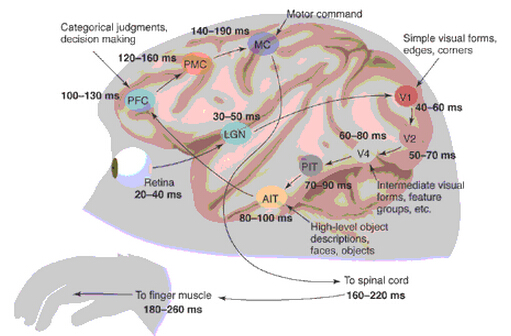
\includegraphics{Pictures/Introduction/brain_flow.jpg}
\caption{可视化刺激任务的大脑通路\cite{thorpe2001seeking}}
\label{Fig:brain_stimulate_flow}
\end{figure}



\section{P300信号检测}\label{sec:introduction_p300}

P300信号是人脑EEG信号中的波形, 受任务相关事件刺激而产生。 激发出P300信号的经典方法是通过“oddball task”产生, 即在一个任务中出现两种模式随机出现, 一种是频繁出现的, 另一种是很罕见的模式。 在任务中, 给定一个刺激,并指导试验个体给出刺激所属模式, 同时采集试验个体的EEG信号, 罕见模式出现时对应的脑信号为P300信号。 例如, 在字符拼写任务中, oddball task是一个关于字符注意的实验(如图\ref{Fig:P300_brief}\cite{polich2007updating}),展现一串字符(如SSTSSSSTSS),其中出现频率高的称为标准刺激(如该信号序列中的S),频率低的称为异常刺激(如该信号序列中的T)。当出现一个异常刺激时,300ms后就会在EEG信号中产生一个正向偏移点位。这里标准刺激和异常刺激的差异可以用来识别所给刺激的类别,然后基于刺激发送信号给计算机指令执行。
 
\begin{figure}[htb]
\centering
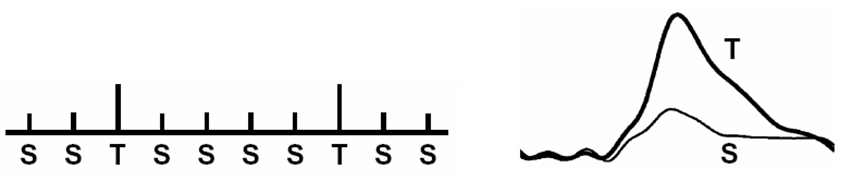
\includegraphics[scale=0.6]{Pictures/Chap1/p300_example.png}
\caption{P300刺激信号. 标准刺激(S)中的异常刺激(T)\cite{polich2007updating}}
\label{Fig:P300_brief}
\end{figure}


1988年 L. A. Farwell 和 E. Donchin 第一次用oddball task建立BCI系统\cite{farwell1988talking}。 该系统中,将36个字符展现在一个6*6的矩阵中, 矩阵的行和列随机闪烁, 同一时刻只有一行或一列亮起,具体哪一行或哪一列是随机的。 如图\ref{Fig:p300matrix}所示, 当一行一列相继闪烁的交点为指定字母时, 测试者可以集中精神在头脑中进行简单计数或者确认, 相应就会有P300在该位置产生, 可以通过估计算法检测到这个P300信号。 也就是说, 如果在对应字母闪烁300ms后在某个位置检测到了P300信号, 就说明主体正在注意这个特定位置。 所以P300的检测实际上就是主体关注位置点字符的检测。  

\begin{figure}[htb]
\centering
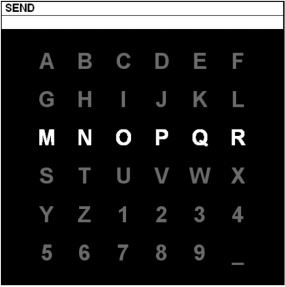
\includegraphics[scale=0.8]{Pictures/Chap1/p300_matrix.jpg}
\caption{oddball task实验矩阵\cite{cecotti2011convolutional}}
\label{Fig:p300matrix}
\end{figure}

在P300检测中, 需要先后两个过程。 第一步, P300位置检测。 这是一个二类分类问题, 给定一个时间段的信号, 判断是否为P300波形。 这个是在实验中进行标注的。 比如, 主体确定了当前要关注的字符, 给定固定顺序随即闪烁行列的矩阵, 我们就可以根据闪烁次序知道当前是否闪烁指定字符, 即是否预期产生P300波形。 但由于一些人为因素干扰, 测试主体不一定能在指定时刻真的给出P300响应, 所以第一步的目标是对这个带噪声的数据进行分类。 第二步根据第一步的分类结果, 对是P300的信号分类属于36个字符中的哪一个。


\section{研究问题与目标}

本文中, 我们将分别用到两种BCI采集到的信号。 脑机接口可以分为侵入式和非侵入式,非侵入式方法,如头皮电信号(scalp electroencephalogram,EEG)易于获取,但是信号精度很差,采样率也相应很低。相反,侵入式脑机接口用外科手术的方法将电极植入大脑皮层进行信号采集,可以采集到很高精度的细胞外神经元信号。在单个神经元中这种高精度信号包含神经锋电位(spike),或者叫做动作电位(action potential)。当神经元被激发的时候就会在神经元膜上产生离子电流,导致细胞去极化(depolarize)并激发出一个spike信号。

本文的研究内容主要有, 侵入式脑机接口的信号压缩, 以及非侵入式脑机接口的信号解码中的一种任务——P300信号检测。 对于侵入式脑机接口, 有信号采集难, 信号采样率高的问题, 导致传输与存储困难。 已有一些工作关注非侵入式脑机信号的采集压缩, 如Electromyography(EMG)和Electroencephalography(EEG)信号的压缩\cite{24,25},为了有效压缩,他们都结合了所处理信号的信号特性, 但是侵入式胞外信号与之相差甚远。 原因是非侵入式信号采集自头皮, 有效信号只在低频部分, 所以可以通过在频域低通滤波进行很大程度上的信号压缩, 但侵入式信号中含有高频spike信号, 难以简单过滤, 使该任务更富有挑战性。 Chen等人对老鼠的S1区域进行研究,通过自适应信号量化在信噪比保持25db的时候达到的压缩率高于25\%,那么信号压缩率和信号质量都得不到保证。 本文中, 我们在浙江大学求是学院BCI系统 \cite{14}上进行植入式运动皮层信号的信号压缩。

对于非侵入式脑机接口, 已有很多相关工作在P300检测方面进行研究, 包括基于SVM\cite{rakotomamonjy2008bci}, LDA\cite{breiman1996bagging}, ICA\cite{yang2008p300}和卷积神经网络\cite{felzer2003analyzing,anderson1995determining,cecotti2008time,masic1995neural,masic1993neural}的方法等。 近年来, 深度学习方法凭借可训特征(或可训的kernel)优势,在语音识别, 图像处理, 声音合成, 生物信号分析等方面超过了手工定义特征的传统方法, 借助现代计算机计算能力的提高和大数据量的爆发得以广泛应用。 本文中, 也采用深度学习的方法进行EEG信号建模, 提高其对P300波形检测效果。 这里我们采用两种模型: 卷积神经网络和循环神经网络模型。 对于卷积神经网络, 已有相关工作进行建模并达到较好的P300检测效果, 但在其模型中有很多部分可以进行改进。 在我们的ConvP300Net方法中, 通过改进模型结构, 可以更好地利用信号空间相关性; 通过重新设计对数据不均衡问题的处理方法, 可以使模型更好地拟合所用数据, 而不需考虑模型集成问题带来的识别增益; 此外ConvP300Net中还加入了很多模型调整部分与方法优化。 对于循环神经网络, 目前很少有方法对非侵入式信号进行处理, 但我们注意到循环神经网络, 尤其是其中的长短时间记忆方法, 可以很好地利用时间维度相关性对时间序列进行建模, 同时避免了传统循环神经网络训练难以收敛的问题。 因此, 本文中设计了LSTMP300Net, 采用长短时间记忆方法对EEG信号建模 , 使其能够更好地拟合信号在P300检测任务上的信号特性。 


之所以分别对侵入式脑机信号和非侵入式脑机信号进行不同任务(压缩和解码), 主要是为了提高问题难度。 侵入式脑机信号难以有效压缩, 且信号采集难度大,对平台有要求,有一些工作分别结合自己的BCI平台进行侵入式脑机接口压缩, 但非常依赖所采集的信号;  非侵入式脑机信号噪声大, 难以进行信号解码, 已有很多工作结合机器学习提出了非侵入式脑机接口神经解码方法, 深度学习的方法虽然在其中占比不高, 但可与一些已有工作进行比较。 所以我们分别在这两种数据上进行信号压缩与解码, 提高研究问题的挑战性。 


本文的目标是, 在侵入式脑机信号的压缩方面, 在保证信号重建质量的基础上提高压缩性能, 使之超过传统数据/文档压缩方法; 在非侵入式脑机信号的P300波形监测方面, 分别采用ConvP300Net和LSTMP300Net超过已有基于神经网络的检测方法。  对于ConvP300Net, 我们在已有相关工作上进行改进, 着重考虑模型调整, 更好地利用信号在空间维度的相关性以及如何直接在网络中考虑各类样本数差异所带来的数据非均匀问题。 对于LSTMP300Net, 我们基于长短时间记忆方法提出了该模型, 并调整网络结构以得到最佳P300波形检测效果。



\section{文章结构}

本文的组织结构如下: 在第二章中, 我们针对侵入式神经信号占用空间大, 传输困难的问题对其进行压缩, 提出了一个新颖的压缩框架, 并在猕猴上采集的神经电信号数据上证明了其有效性。 之后, 我们在非侵入式EEG信号上采用深度学习的方法进行P300检测中的第一个环节,即 检测一段信号是否是P300信号。 第三章和第四章分别采用卷积神经网络和循环神经网络对其进行建模, 构建了ConvP300Net和LSTMP300Net并分析模型的有效性。 这里之所以在压缩部分采用侵入式脑机接口所得神经电信号是因为项目平台需要。 侵入式神经电信号的高精度高采样率决定了其大数据量, 阻碍了在我们的信号采集平台中的快速传输, 需要对其压缩, 而现有神经信号压缩方法都会使信号失真, 所以需要针对我们所采集的信号特性进行高保真神经电信号压缩。 而第三、四章在神经解码应用中我们采用的是非侵入式方法所得的EEG信号, 这是出于方便与其他模型比较考虑的。 在三、四章中, 我们采用公开BCI竞赛数据集\cite{blankertz2006bci}, 已有很多包括神经网络在内的方法应用于该数据集以提高神经信号解码效果, 采用该数据集方便我们进行合理的模型比较, 而据我们所知, 侵入式脑电信号没有公开竞赛数据集。











\chapter{侵入式神经信号压缩方法}

在侵入式脑机接口(invasive Brain Machine Interface)中,我们将多电极阵列(multi-electrode array, MEA)植入大脑皮层从而获取高质量的电神经信号。 这种信号的采样率为30kHz, 给数据存储和传输带来了重大负荷, 所以我们需要对数据进行压缩来降低数据量。在这一节中,我们结合大脑运动皮层神经电信号的特性,提出了一种高保真压缩算法。实验中,我们将该算法应用于哺乳动物的大脑运动皮层信号,相对原信号得到了18\%的压缩率,而且没有对信号重建产生明显影响。该方法的信噪比(signal to noise ratio, SNR)达到36dB,而且spike信号也保存下来92\%,大幅超过已有工作的效果。 本章工作发表在IJCNN 2014\cite{zhang2014high}.

\section{神经电信号(electroneurographic signal)}

本章中我们将主要关注运动皮层神经信号。作为大脑皮层的一个重要部分,运动皮层负责计划,控制并执行人体主动行为。在运动皮层功能的相关研究中,电极阵列所采集的多通道信号通常在每个通道进行分频。通道中信号低频部分(截止频率在100Hz)对应神经信号的局部场电位(local field potential, LFP),而中频到高频部分对应于动作电位(spikes)。LFP主要源于前突触行为,反映了很多树突行为的平均电流。与之相反,Spike主要反映兴奋神经元的行为。LFP和spike信号对神经解码都很重要。对于运动皮层而言,spike通常的持续时间小于1毫秒,因此需要用高分辨率设备进行信号采集。这里我们用多电极阵列刺入细胞去采集数以百计的感兴趣神经元的信号。哺乳动物运动皮层神经元信号通常以20-30kHz的频率采集128个通道,以保证可以完好保存spike细节。这样,以16-bit的A/D分辨率计算,如果采样率为30kHz,那么128个通道的信号就会以7.68MB/s的速度进行采集。换句话说,一小时内的信号量就积累到28.8GB,这对信号的存储和传输都带来了巨大挑战。所以,我们要对信号进行压缩。

尽管BMI系统已经建立得比较完善了,脑皮层胞外信号的记录并没有深入研究过。在Electromyography(EMG)和Electroencephalography(EEG)信号的压缩上有过一些相关工作\cite{},为了有效压缩,他们都结合了所处理信号的信号特性。但是侵入式胞外信号与之相差甚远。

现有多通道压缩算法从两种思路进行实现。一种是应用通道内特性对每个通道的信号分别进行压缩,另一种是用通道间相关性同时对所有通道的信号进行压缩。从第一个思路出发,Weber等人通过基于小波的编码器对老鼠躯体感觉皮质(S1区)进行压缩,然后这种方法代价是丢掉了25\%的spike,对于后期的信号还原和分析并不理想。Chen等人对老鼠的S1区域进行研究,通过自适应信号量化在信噪比保持25db的时候达到的压缩率高于25\%,那么信号压缩率和信号质量都得不到保证。为了改善他们的工作,Chen从第二种思路出发,利用通道间的信号相关性,在25db信噪比的情况下,将压缩率降至5\%。然而,以上几种方法都丢失了太多信号细节,白费了采集来的高分辨率信号。

本章中,我们提出了一个运动皮层胞外信号的高保真压缩框架。 首先,我们讨论这种信号的3个特性:1) 信号能量集中在低频;2)离散余先变换系数中的高频部分可能对英语spike的激活模式 3)通道间相关性不稳定。根据特性(2),我们提出了一个新颖的幅值滤波器,将离散余先变换系数按幅值,而不是按频率分为两部分。低幅值成分由一个符号编码方法进行编码来降低全局失真;高幅值成分,包含主要信息和spike,由另一步骤编码。这个步骤叫混合编码,包含哈弗曼编码和一个新颖的零长编码。我们的主要工作如下:

\begin{list}{-}
\item 设计了一种新颖的幅值滤波器,它将离散余先变换系数根据幅值分为两部分,这避免了spike信息的丢失。
\item 提出了一个符号编码方法,用来对低幅值成分进行编码,而不是简单丢弃。这有效避免了全局信号失真。 
\item 发明了一种合并哈弗曼编码和新颖的零长编码的混合编码方法,用来对高幅值成分和低幅值成分的索引进行编码。由此,spike信息得到了精准的结构化保存。
\end{list}




最后,我们用一系列方法测试我们提出的压缩框架,得到了平均信噪比36db,压缩比18\%的效果,而且spike保真率保持在92\%以上,保证了重构效果。





\section{运动皮层胞外信号特点}\label{sec:characteristic}


为了在保证信号质量的同时进行有效压缩,我们在本节中多通道胞外信号的特点。我们的数据将在实验部分进行详细描述。这里,我们从通道内特点到通道间相关性,总结出三个特点:

\begin{enumerate}
\item{信号能量集中在低频:}\\
为了研究所记录信号的频域特性,我们采用离散余弦变换(discrete cosine transformation, DCT)将数据先转换到频域。作为傅里叶变换的一个变种,DCT系数得到的是一系列实数,处理起来比傅里叶变换方便。变换后的DCT系数用${x_i} = [x_i^{1},x_i^{2},...,x_i^{N}]$来表示,其中$x_i^j$表示第i个通道DCT系数中的第j个元素。那么整个数据集上低频部分能量比例为:

\begin{equation}\label{Eq:power Definition}
  P = \frac{\sum_i \|x_i^{1},x_i^{2},...,x_i^{T_{p0}}\|_2}{\sum_i \|x_i\|_2}
\end{equation}
 
式中,分母表示所有通道总能量,分子为所有通道的前Tp0个DCT分量的总能量,即,以Tp0为截止频率,低频部分的能量。在整个数据集上,我们将P的平均值画在图\ref{Fig:Characteristic1},图中横轴$T_{p0}$ 表示计算几个元素的能量和,纵轴表示前$T_{p0}$个元素的能量和占比, 这清晰表明了少量DCT分量占据了信号的主要能量。换句话说,相当大的能量集中在了低频部分。

\begin{figure}
  \centering
  % Requires \usepackage{graphicx}
  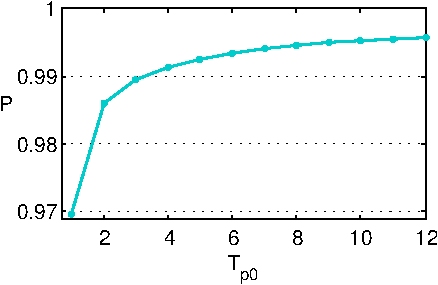
\includegraphics[width=3in]{Pictures/Compression/f1-crop.pdf}\\
  \caption{频域前12个系数的能量分布。}\label{Fig:Characteristic1}
\end{figure}


\item{高频信号中存在显著峰值:}\\
和其它自然信号(如图像)一样,胞外信号的主要能力也集中在低频部分。然而,这样的信号在中高频有所差异。如图\ref{Fig:Characteristic2}所示为中频部分的一部分截断光谱,可见在7325Hz处有一个明显的峰值,对应于一个经常出现的神经元放电模式。实际上,实验表明很多通道共享这些具有峰值的频率,而一些通道没有。这可以从多电极阵列的采样原理理解,我们采集到的胞外信号的单通道信息可以由3至5个有不同spike激发模式的神经元组成。

\begin{figure}[htb]
  \centering
  % Requires \usepackage{graphicx}
  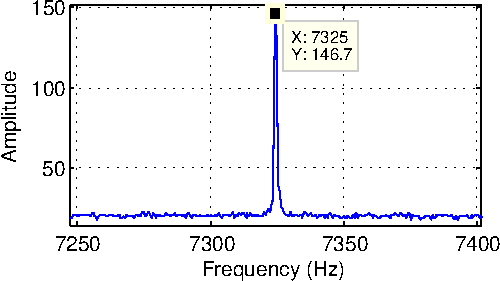
\includegraphics[width=3in]{Pictures/Compression/f2-crop.pdf}\\
  \caption{神经电信号高频部分DCT系数幅值分布。}\label{Fig:Characteristic2}
\end{figure}


\item{不稳定的通道间信号相关性:}\\
在\cite{chung2008intelligent}的工作中Chen等利用了老鼠S1区采集信号的通道间相关性达到了较高的压缩效果。受此激发,我们也来研究一下在哺乳动物的运动皮层是否存在这样的相关性。

将原信号分为10个等长连续段,用$\bm{F}=\bm{\{F^1, F^2,\ldots, F^{10}\}}$表示这10段在频域的平均DCT系数,$\bm{F^{i}}\in R^{N_c\times S_b}$表示第i段的平均DCT系数大小,$N_c$为channel数目,$S_b$表示待转换为频域的信号长度。对于每个$\bm{F^{i}}$,我们计算其两两通道间的相关系数,记$\bm{C} \in R^{N_c\times N_c}$。图\ref{fig:Characteristic3}(a)(b)显示了一个时间序列段内频域的96个通道的两两相关系数矩阵,矩阵中,(i,j)位置的值表示 $i_{th}$ 通道和 $j_{th}$ 通道之间的相关系数,越深表示相关性越大,可见相关性变化很大。用变换系数(coefficient of variation)衡量相关系数的相对离散程度:


\begin{equation}\label{Eq:CV Definition}
  CV=\frac{\sigma}{\mu}
\end{equation}


其中 $\sigma$和 $\mu$分别表示相关系数的标准差和均值。当一个信号的$\sigma$相对$\mu$可忽略不计时,即CV很小时,称信号为稳定信号。对每个时间段$\bm{F^{i}}$,$\bm{CV}\in R^{N_c\times N_c}$衡量相关矩阵\textbf{\emph{C}}的浮动区间。$CV$的均值显示在图\ref{fig:Characteristic3}(c)中, 它是数据集中所有时间序列段内$CV$矩阵的平均值。 (i,j)位置的高度表示$CV$矩阵中$i_{th}$ 通道和 $j_{th}$ 通道相关系数的平均值。 这$N_c\times N_c$个$CV$的均值为0.68, 也就是说, 相关系数随时间剧烈变化, 所以在我们获得的运动皮层神经信号中, 通道间的相关性并不稳定,所以也较难将其应用在减少通道间冗余上。


\begin{figure}
  \centering
  % Requires \usepackage{graphicx}
  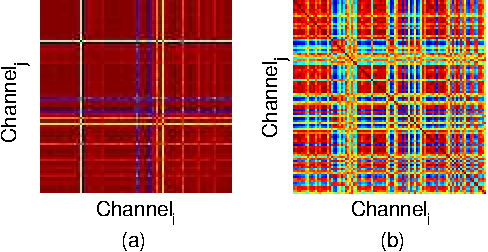
\includegraphics[width=3in]{Pictures/Compression/f3(ab)-crop.pdf}\\
  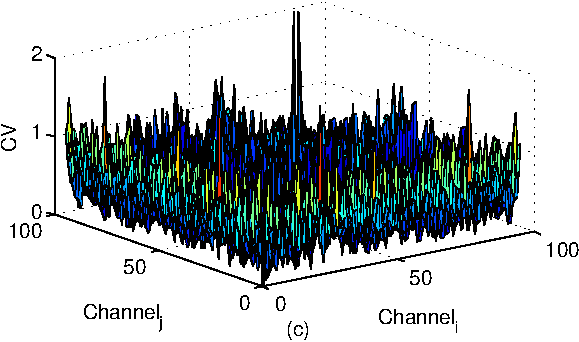
\includegraphics[width=3in]{Pictures/Compression/f3(c)-crop.pdf}\\
  \caption{通道间相关系数。 }\label{fig:Characteristic3}
\end{figure}

\end{enumerate}



\section{提出方法概括}
这篇文章中,我们考虑到上述信号特征,提出了一个高保真神经电信号压缩框架。首先,由于通道间相关性不稳定,我们对每个通道的信号做独立处理。整个框架的示意图见图\ref{Fig:Compression Algorithm Diagram}。它包括两个连续模块:"预处理"和“双阶编码”。

\begin{figure*}
  \centering
  % Requires \usepackage{graphicx}
  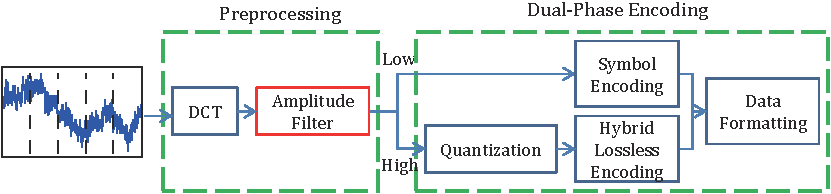
\includegraphics{Pictures/Compression/f4test1-crop.pdf}\\
  \caption{Flow diagram of the overall compression algorithm}\label{Fig:Compression Algorithm Diagram}
\end{figure*}

对于每个通道,首先将原信号分割成长度为$S_b$的块,然后每块通过以下两个模块进行处理:\\
\begin{enumerate}[\sffamily a.]
\item{\textbf{\textit{Preprocessing}}}\\
该模块通过离散余弦变换(Discrete Cosine Transformation,DCT)将原信号转换成频域。由于高频部分一些峰值可能对应于spike firing模式,所以传统压缩方法不适用于该信号的压缩。因此,我们提出按频谱幅值对信号进行分割,而不是根据频率高低分割。DCT系数通过一个幅值滤波器,分为高幅值成分(High-Amplitude-Component,HAC)和低幅值成分(Low-Amplitude-Component,LAC)。HAC包含显著地LFP和动作电位,其他信号归入LAC。 
 
\item{\textbf{\textit{双阶编码}}}\\
在神经信号的研究分析中已有证明,一个神经元完全由其神经元受刺激后的信号发放频率firing rate刻画\cite{32}。信号发放频率为单位时间内的动作电位发放个数。这个概念在2007年被\cite{3}中做出了修正,其中声明将LFP和spike结合起来可以加强神经信号解码准确率。也就是说,高幅值成分对神经信号表达更重要,因为这部分包含LFP和spike活动。相反,低幅值部分有效性较弱,但我们为了全局信号保真度和后续研究,也应在压缩时予以保存。这里我们提出双阶编码模块,它可以同时保存HAC和LAC的信息。在第一个阶段,低幅值部分由符号编码进行压缩,每个LAC中的DCT系数由1bit的符号表示;第二个阶段中,先将高幅值部分量化到一个相对小的范围区间,在通过我们提出的无损混合编码策略进行压缩。
\end{enumerate}









\section{双阶编码}
双阶编码模块的提出就是为了在压缩过程中同时保存全局和局部神经电信号。它对预处理信号定义了两个独立的操作。第一个阶段采用有损压缩策略,通过符号编码压缩低幅值部分,在这个阶段,16bit的原始信号值通过平均值平滑由1bit的符号表示。在第二个阶段,将DCT系数中LAC部分置零。所得到的向量中包含HAC部分量化后通过一个混合编码方法进行压缩。该编码方法将哈夫曼编码和我们提出的零长编码进行混合。哈夫曼编码处理高幅值项,而零长编码处理向量中的零元素。通过混合编码对LAC和HAC分开压缩可以有效地保存LAC和HAC的频谱位置,而无需存储多余信息。最后,对这两部分生成的编码进行格式化存储。
 
 
 
\subsection{符号编码}
\label{sec:symbol_encoding}
在双阶编码模块的输入端,信号通过一个幅值滤波器。为了达到高压缩率,低幅值部分通常直接被舍弃。但这样的话大块丢弃的系数容易引发很大重构误差,从而影响信号保真度和后续研究。为了解决这个问题,我们为该部分提出了一个有效的表示方法。

在神经信号解码的研究中,从带噪声的数据中预测神经元响应是一大难题:给定相同的刺激,但神经元几乎没有两次会出现相同的活动模式。为了准确表示神经元表达,需要对信号做一些均值平滑处理 \cite{31}。因此,均值通常用来代表原始系数,受这个激发,我们这里也在压缩过程中用信号的均值代替。

在符号编码中,均值在频域进行操作。低幅值DCT系数用其均值表示。由于正负系数进行平均可能被抵消,因此我们存储的是幅值,即系数的绝对值。为了有效压缩,各通道LAC部分的平均幅值预先计算好,然后用1-bit的符号表示其正负。记LAC中元素i为$l_i$,其符号表示为:

\begin{equation}\label{Eq:symbol definition}
  symbol(l_i)=\left\{
    \begin{array}{lr}
        -1,\ -T_{LH}<l_i\leq 0\\
        1,\ 0<l_i<T_{LH}
    \end{array}
  \right.
\end{equation}

其中-1,1位系数符号,-1示负,1表示正,$T_{LH}$表示低幅值和高幅值之间的分界阈值。根据公式\ref{Eq:symbol definition},含有$S_l$个元素的LAC向量通过符号编码被压缩为$S_l$个bit的向量,用来在解码时恢复。

在压缩解码时,我们将每个元素的编码符号乘以其幅值即可。这里有一个问题就是如何恢复LAC部分元素的位置。我们可以直接存储其位置,但是这样太耗费空间。事实上,我们无须显式存储其位置。由于LAC部分已经被编码,我们可以在待压缩信号中将其置零,而后续处理中只要保证其他压缩元素都非零即可,这样,在解码时只要找出所有零项即可恢复LAC。



\subsection{量化}
由于HAC部分包含LFP和主要spike,这个重要部分要比LAC做更精细的保存。为此,这一块信息线被量化到一个小区域,然后通过一个混合编码方法进行压缩。本节中介绍第一步操作——量化。当信号从预处理模块输出是,每个长为$S_b$的数据块通过一张量化表进行量化。这本身是一个有损压缩过程,但是通过共享量化表可以丢掉部分冗余信息。量化定义为原始信号除以对应的量化值,然后取整。这些量化值在不同信号通道又不同取值,从而组成量化表(Quantization Table, QT)。令$QT\in R^{N_c\times S_b}$表示量化表,其中$N_c$表示通道数,$S_b$表示数据块大小。记量化后第c项为$H_c^Q$,有

\begin{equation}\label{Eq:Quantization Step}
  H_c^Q=round(H_c./QT(c,:)),
\end{equation}

其中./是一个向量逐项除法,$round(x)$为取整操作,返回距离x最近的整数。注意,$H_c$中的元素幅值都大于等于$T_{LH}$,所以只要能令$ QT(c,:)$中的元素都小于$T_{LH}$,那么量化后,HAC的绝对值就都大于等于1了,这样可以很好地分离压缩后信号中的LAC分量和HAC分量。

对于待量化的高幅值部分,其取值范围由信号和$T_{LH}$共同决定。然而,神经电信号会因个体差异而拥有不同的采集信号取值\cite{33}。而且,不同神经元拥有不同的频谱分布,因此需要对每个个体的不同通道建立特定量化表。在符号编码中我们已经计算了LAC的平均幅值,这里我们将其用于量化表。

该量化表的设计出于以下几点考虑。一,考略到个体差异性,我们给每个实验个体建立独一无二的量化表。二,我们在研究运动皮层神经电信号特性时讲到过不同通道具有不同皮普分布,因此量化分量在通道间不共享。三,由于取整操作,转换后的取值有所变化,但是变化幅度不会大于对应位置量化值的$\frac{1}{2}$,不会损失太多信息。而且,这样量化表的值也可以都小于$T_{LH}$,使得量化后结果不小于1,满足了\ref{sec:symbol_encoding}节中提到的非零特性。



\section{混合无损编码}
由于高幅值部分所有元素在量化后都成为了整数,离散分布的信号可以通过编码无损压缩,该无损压缩可由哈夫曼编码和零长编码方法实现。

作为最优符号编码方法,哈夫曼编码生成最佳可变长码,可以有效运用在我们量化后的数据上。然而,很多高频部分DCT系数的幅值都很小,容易被归入LAC分量。经过幅值过滤器处理后,很多高频参数在HAC中变成了0.因此,可以通过将高频部分连续的0替换成0的个数达到更好的编码效果,这就是零长编码的思想。于是,所有非零DCT系数都可以与哈夫曼编码表示;设置一个界限$B$,$B$之前的零用哈夫曼编码方法,$B$之后的零用零长编码分别进行表示。为了有效结合这两种方法,$B$的设定就很重要了,而它的取值取决于零的分布。为了更清晰地描述我们提出的混合编码方法,我们首先介绍一下哈夫曼编码和零长编码,然后来看怎样设置临界点$B$。


\subsection{Huffman编码}
熵编码方法是一种无损压缩技术,通常为每个符号创建一个独一无二的码。作为最常用的熵编码方法,哈夫曼编码\cite{22}用在我们的无损编码部分,旨在建立一棵最优树,能够最小化加权树高和(即信号编码总长度)\cite{21}。为了将原始值转换成二进制序列,哈夫曼编码方法基于每个符号的出现次数进行编码。

首先来看计算DCT系数的分布。根据我们的实验,HAC系数服从高斯分布,而很高的幅值非常少,那么为所有系数建立哈夫曼编码就是一件既耗时又浪费空间的做法,因为首先要计算其哈夫曼编码,而后由于其频率太少,会导致码字很长,浪费空间。因此我们并非计算所有DCT系数分布,对于非零系数,我们只计算$[-Z,Z]$的部分,其中$Z$是系数的统计范围。而超出该范围的幅值,我们单独记录其值和位置。此外,并非所有系数零都予以统计。令\emph{B}表示哈夫曼编码与零长编码之间的分界点,由于只有\emph{B}之前的零采用哈夫曼编码,我们就只统计\emph{B}之前出现的零的个数。




\begin{figure}
  \centering
  % Requires \usepackage{graphicx}
  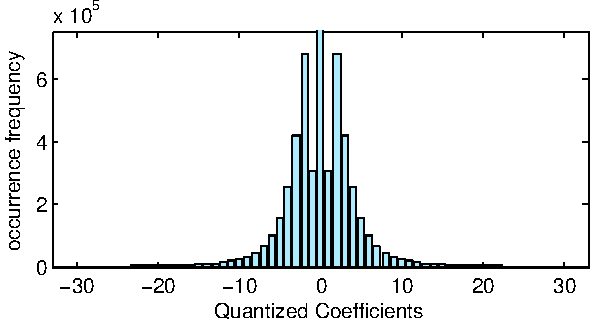
\includegraphics{Pictures/Compression/f5-crop.pdf}\\
  \caption{频域量化系数。}\label{fig:Quantized Coefficient Distribution}
\end{figure}


统计幅值在$[-Z,Z]$内所有非零系数以及$B$Hz前零元素的分布,将$N_c$个通道求得平均,如图\ref{fig:Quantized Coefficient Distribution}所示, 其中横轴表示[-31,31]的整数系数范围,纵轴表示量化后每个系数的出现次数。在这个例子中,$B$由\ref{sec:delimerate}节中的定界策略决定。根据这个统计结果,哈夫曼编码对这些系数进行编码。



\subsection{零长编码(Zero-Length-Encoding)}
\label{Zero-Length-Encoding}

零长编码方法为了对高频部分连续的零进行编码。我们用八进制表示法表示连续$k_z$个零,用哈夫曼编码来分隔两个相邻的八进制数字。举例,$k_z=(8A+B)\times 8+C$,其中$A$, $B$, $C$ 分别表示三阶,二阶,一阶的八进制数字。用\textbf{\emph{HCT}}表示哈夫曼码表(Huffman Code Table), 即DCT系数的不定长编码表,混合编码格式如下:

\begin{figure}[H]
  \centering
  \caption{混合编码格式示例}
  % Requires \usepackage{graphicx}
  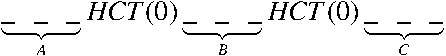
\includegraphics{Pictures/Compression/HCT-crop.pdf}\\
\end{figure}

令$g(k)$为要表示的0个数所需阶数,我们有


\begin{equation*}
  g(k_z)=\left\{
    \begin{array}{lr}
        1,\ k_z\in[0,7]\\
        2,\ k_z\in[8,7\times8+7]\\
        3,\ k_z\in[64,63\times8+7]\\
        \ldots
    \end{array}
  \right.
\end{equation*}


可以规范化为:
\begin{equation}\label{Eq:g(kz) definition}
  g(k_z)=\left\{
    \begin{array}{lr}
        1,k_z=0\\
        \lceil \log_8(k_z+1) \rceil,else
    \end{array}
  \right.
\end{equation}

在解码过程中,首先读入一个3-bit二进制码字,然后检测下一个序列是否和$HCT(0)$相同。如果是,就再读三位,以此类推,直到条件不满足为止,这时就可以计算该段有多少个连续0了。由于哈夫曼编码是前缀无歧义编码(prefix-free code), 所以可以保证零的表示不会出现歧义。

零长编码通过直接编码连续零,而非一个个表示来节省空间,因此我们希望零长编码的信号段拥有更多连续的零(而不是分散的),因此确定一个好的分界点$B$尤为重要。








\subsection{混合无损编码分界}\label{sec:delimerate}
随着量化信号中连续零数量的增多,可以想见零长编码要比哈夫曼编码短,为了证实这个想法,我们来看混合编码策略中两种编码方法的编码。

对分界面的简单估计可以通过计算零的个数分布而得。将每$S_b$个离散时间序列点分为$N_s$个等长短序列段,然后计算每段中零的个数。图\ref{fig:Zero Distribution}显示了1600个DCT系数分割为16段($S_b$=1600, Ns=16)的零数分布, 对于 $S_b=1600$, 将1600个元素分为16段,每段有100个分量。黄色和蓝色线条分别表示每段中零元素个数的均值和方差。 可以看出零的个数分布随着频率而增多。用$\Omega_0\in R^{N_s}$表示平均零数分布,即图中的黄色条,则可以根据零数分布情况进行分界。

\begin{figure}
  \centering
  % Requires \usepackage{graphicx}
  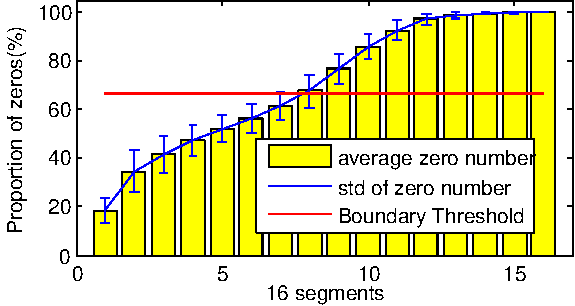
\includegraphics{Pictures/Compression/f6-crop.pdf}\\
  \caption{16个序列段的零元素分布情况。}\label{fig:Zero Distribution}
\end{figure}

令$T_{HZ}$表示在哈夫曼编码与零长编码的分界$B$处,零的出现概率,那么该段中领的个数可以用$T_{HZ}\cdot \frac{S_b}{N_s}$表示,其中$\frac{S_b}{N_s}$是每段中的元素个数。这样,分界限可由式\ref{Eq:Boundary Brief Def}得出,$B$之前采用哈夫曼编码,$B$之后采用零长编码。

\begin{equation}\label{Eq:Boundary Brief Def}
  B=CrossSegment\left(\Omega_0,T_{HZ}\cdot\frac{S_b}{N_s}\right)\cdot\frac{S_b}{N_s}
\end{equation}

该式中,CrossSegment函数返回零的出现频率和阈值$T_{HZ}$的交点出数据段编号。图\ref{fig:Zero Distribution}中红色线表示阈值$T_{HZ}*(S_b/N_s)$,用来分隔混合编码中的两个算法, 图中可见零分布线(黄色)与阈值线(红色)交于第7段。该例中,$S_b$=1600, $N_s$=16, 定义 $T_{HZ}$=0.75,那么有$B$=700。


下面我们来仔细分析交点位置。用x表示交点段的编号,在式\ref{Eq:Boundary Brief Def}中直接用$T_{HZ}$乘以每段中的元素个数,而在式\ref{Eq:Boundary Precise Def}中,考虑到了交点段中阈值与段交点处所占的比例。


\begin{equation}\label{Eq:Boundary Precise Def}
  \begin{array}{lr}
    x=CrossSegment\left(\Omega_0,T_{HZ}\cdot\frac{S_b}{N_s}\right)\\
    B=\left((x-1)+\frac{T_{HZ}\cdot \frac{S_b}{N_s}-\Omega_0(x-1)}{\Omega_0(x)-\Omega_0(x-1)}\right)\cdot \frac{S_b}{N_s}
  \end{array}
\end{equation}


最后一个问题是$T_{HZ}$的设定。由于$T_{HZ}$表示在$B$处,系数零所占比例,它可以表示每个非零元素之前平均零的个数,即


\begin{equation}\label{Eq:T_HZ def}
  T_{HZ}=\frac{k_z(B)}{k_z(B)+1}
\end{equation}


其中的1表示非零系数,$k_z(B)$表示在分界线$B$处一个非零系数之前的平均零的个数。

基于DCT系数的统计特性,分界可以进一步提升压缩性能。然而,从上面的推导可知,在式Eq.\ref{Eq:Boundary Precise Def}和 \ref{Eq:T_HZ def}中,计算$B$和$T_{HZ}$是一个死锁。公式\ref{Eq:Boundary Precise Def}需要$T_{HZ}$的值,而$T_{HZ}$的值要在式\ref{Eq:T_HZ def}中由\emph{B}决定。为此我们提出了一个迭代检验方法,该法需要根据混合编码两种方法生成的码字长度合理确定界限的位置。

令$HCT$表示前面生成的哈夫曼编码表,
\textbf{\emph{HCT}}(x)表示x的哈夫曼编码,
$l_0\in Z_+$ 表示$HCT$码表中0的码字长度,
$k_z$ 表示一个非零元素之前0的平均个数。若量化系数全部由哈夫曼编码表示,其长度为:


\begin{equation}\label{Eq:length of Huffman}
  l_1=\sum_{i=1}^I [HCT(x_i)]+l_0\cdot k_zI,\ x_i\in H_c^Q, x_i\neq 0
\end{equation}


其中$I$是$H_c^Q$中所有非零系数集合的大小。该式中,第一项将所有非零元素$x_i$的长度进行加和,
而$l_0\cdot k_zI$ 表示所有‘0’的长度和,因为每个非零系数之前平均有 $l_0\cdot k_z$ 位数字。


类似地,如果量化系数中的零全部由零长编码表示的话,编码长度为:


\begin{equation}\label{Eq:length of Zero-length-Encoding}
  l_2=\sum_{i=1}^I [HCT(x_i)+(3+l_0)g(k_z)-l_0],\ x_i\in H_c^Q, x_i\neq 0
\end{equation}


根据零长编码格式\ref{Zero-Length-Encoding},$(3+l_0)$是八进制表示中每多一阶多需要的表示位数。用 $g(k_z)$ 表示$k_z$个零所需阶数,则 $(3+l_0)g(k_z)-l_0$ 可以表示一个非零元之前的零分量用零长编码所需长度。此处$k_z$并非确切平均零的个数,而是为了计算方便估计的最近整数。

To compare the two encoding length, we use Eq.(\ref{Eq:length of Huffman}) minus Eq.({\ref{Eq:length of Zero-length-Encoding}}) and take the part in the bracket as $f(k_z)$,

为了比较两种编码方法的长度,我们用公式\ref{Eq:length of Huffman}减去式\ref{Eq:length of Zero-length-Encoding},计入下式方括号内,即$f(k_z)$:


\begin{equation}\label{Eq:length difference}
  l_1-l_2 = \left[l_0\cdot k_z-(3+l_0)g(k_z)+l_0\right]I=f(k_z)\cdot I
\end{equation}


由于I是常数,我们只考虑以$k_z$为参数的函数f。将式(\ref{Eq:g(kz) definition}) 代入式(\ref{Eq:length difference}), 我们有


\begin{equation}\label{Eq:f(kz) Def}
  f(k_z)=\left\{
    \begin{array}{lr}
        -3,\ k_z=0\\
        l_0\cdot k_z-(3+l_0)\lceil\log_8(k_z+1)\rceil+l_0,\ else
    \end{array}
  \right.
\end{equation}


对于离散整数 $k_z$, 相邻项之间的差为:


\begin{equation}\label{Eq:f(kz)difference}
\begin{array}{lr}
  f(k_z)-f(k_z-1)=\left\{
    \begin{array}{lr}
        f(0)=-3;\\
        f(k_z)=f(0)+l_0k_z-(3+l_0)\lfloor\log_8{k_z}\rfloor
    \end{array}
  \right.\\
  \\
  where \ k_z\in Z_+,l_0\in Z_+
\end{array}
\end{equation}


由式(\ref{Eq:f(kz)difference})可得,$f(k_z)$只有在$k_z$最开始,即$l_0$不大于1时才会小于零。由于随着频率增加,$f(k_z)$有增加的趋势,所以$f(k_z)$与0只有一个交点,就是在 $\lfloor\log_8{k_z}\rfloor$ 等于零的时候。
在这个交点处,我们可得从式(\ref{Eq:f(kz)difference})得:


\begin{equation}\label{Eq:kz}
  k_z=\frac{3}{l_0}
\end{equation}


所以,混合编码中的阈值可以由式(\ref{Eq:T_HZ def})和 (\ref{Eq:kz})确定。 但是在参数选择过程中还有其他问题。正如我们之前提到的,在确定界限$B$,阈值$T_{HZ}$和哈夫曼编码表之中有死锁。
问题在于, $T_{HZ}$ 由 $k_z$ (式(\ref{Eq:T_HZ def}))计算而得,而$k_z$依赖 $l_0$ (式(\ref{Eq:kz})), $l_0$又由哈夫曼码表确定. 然而, \textbf{\emph{HCT}}需要计算 \emph B之前零的个数, 而这又由 $T_{HZ}$得来。为了打破这个死锁,我们再假设$l_0=1$下初始化$k_z$,见Boundary Descent 算法.

\renewcommand{\algorithmicrequire}{ \textbf{Input:}}      %Use Input in the format of Algorithm
\renewcommand{\algorithmicensure}{ \textbf{Output:}}     %UseOutput in the format of Algorithm
\begin{algorithm}
\caption{BOUNDARY DESCENT ALGORITHM}
\label{algo:bda}
\begin{algorithmic}[1]  
\Require Quantized HAC to be compressed $H_c^Q$
\Ensure  \textbf{\emph{HCT}},\emph{B}
\State	$k_z\leftarrow3,\varepsilon\leftarrow1$
\While{($\varepsilon=1$)}
    \For{$c\leftarrow1 to N_c$}
        \For{$i\leftarrow1 to S_b$}
            \State $\Omega_0(i)\leftarrow \sum_{c=1}^C 1_{\left\{H_c^Q[i]=0\right\}}$
        \EndFor
    \EndFor
    \State $T_{HZ}\leftarrow \frac{k_z}{k_z+1}$
    \State $x=CrossSegment\left(\Omega_0,T_{HZ}\cdot\frac{S_b}{N_s}\right)$
    \State $B=\left((x-1)+\frac{T_{HZ}\cdot \frac{S_b}{N_s}-\Omega_0(x-1)}{\Omega_0(x)-\Omega_0(x-1)}\right)\cdot \frac{S_b}{N_s}$
    \State $HCT\leftarrow Huffman Encoding(H_c^Q,B)$
    \If{($l_0(HCT)=\frac{3}{k_z}$)}
        \State $\varepsilon\leftarrow 0$
    \Else
    	\If{($l_0(HCT)\leq 3$)}
    	    \State $k_z\leftarrow \frac{3}{l_0(HCT)}$
    	\Else
	        \State $B\leftarrow 0,\ \varepsilon\leftarrow0$
	    \EndIf
    \EndIf
\EndWhile
\end{algorithmic} 
\end{algorithm}


算法\ref{algo:bda} 描述了界限下降算法的流程。令$\varepsilon$表示是否迭代的标志, $l_0(HCT)$ 表示哈夫曼码表中零编码长度,从假设 $l_0$(\textbf{\emph{HCT}})为1开始, 算法初始化$k_z$ 为3 (第一行)。只要迭代标志为真,就计算所有样本中的零分布(3-7行)。然后通过式(\ref{Eq:Boundary Precise Def}计算该方法的阈值 $T_{HZ}$ (第8行),然后根据式\ref{Eq:T_HZ def})计算混合编码中两种方法的分界点$B$ (9-10行)。以$\emph{B}$和量化信号$H_c^Q$作为输入,可获哈夫曼码表 \textbf{\emph{HCT}}(line 11)。
然后,检验最初的假设,即是否满足式(\ref{Eq:kz}). 如果迭代所得 $l_0$与假设不吻合,就用$\frac{3}{l_0}$代替,始终迭代直到达到条件$l_0$(\textbf{\emph{HCT}})$\cdot k_z = 3$ (12-16行)。注意$l_0$应被限制在3之内,否则就无须用哈夫曼编码了(17-19行)。这个算法最终返回 \textbf{\emph{HCT}} 和分界处 \emph{B}。

\begin{algorithm}
\caption{Overall Compression Algorithm}
\label{algo:overall_algorithm}
\begin{algorithmic}[1]  
\Require {$\bm{X}$, the signal; $S_b$, the block size; $T_{LH}$, the threshold between HAC and LAC; \emph{B}, the boundary within Hybrid Encoding}
\Ensure {$\bm{Y}$, formatted compression result; $\bm{Z}$, lengths of \emph{Symbol Encoding} codes for all blocks }
\State Divide $\bm{X}$ into blocks of size $S_b$, $\bm{X}_{(1)},\bm{X}_{(2)},...,\bm{X}_{(N)}$
%Calculate Quantization Table and LAC\\
    \For{$i = 1,...,N$}
        \State $\bm{F}_{(i)} \leftarrow DCT(\bm{X}_{(i)})$
        \State $\bm{low}_{(i)}\leftarrow$ find indices $(\bm{F}_{(i)}<T_{LH})$
        \State$\bm{LAC}_{(i)} \leftarrow F(\bm{low}_{(i)});\%\emph{LAC}$
    \EndFor
    \State $\bm{QT}\leftarrow$ average over $|\bm{LAC}_{(i)}|$,\,\,$i=1,...,N$
	\State $\bm{Y}$ $\leftarrow$ [\,]
\For{$i = 1,...,N$}
    \State $\bm{HAC}_{(i)} \leftarrow \bm{F}_{(i)}$; \,\,$\bm{HAC}_{(i)}(\bm{low}_{(i)}) \leftarrow 0$
    \State $\bm{S}\leftarrow sgn(\bm{LAC}_{(i)})$;\,\, $\bm{Y}\leftarrow [\bm{Y}\; \bm{S}];$  \%\emph{Symbol Encoding}
    \State $\bm{Z}_{(i)}\leftarrow length(\bm{S})$; 
    \State $\bm{H_c}^Q\leftarrow round(\bm{Hc}_{(i)}./\bm{QT});$
    \State $\bm{H}\leftarrow Huffman(\bm{H_c}^Q(1:B))$; $\bm{Y} \leftarrow [\bm{Y}\; \bm{H}];$
        \ForAll{$x \in \bm{H_c}^Q((B+1):end)$}
        	\If {$x\neq 0$}
            	\State $\bm{Y} \leftarrow [\bm{Y}\; Huffman(x)]$
	        \Else
    	        \State $\bm{Y} \leftarrow [\bm{Y}\; ZeroLength(x)]$
    	    \EndIf    	        
        \EndFor
\EndFor
\end{algorithmic}
\end{algorithm}


通过算法\ref{algo:bda} 求得压缩框架的全部参数后,我们用算法\ref{algo:overall_algorithm}总结一下整个算法的流程。 首先将信号以$S_b$为大小分割成$N$块,对于每个数据块,分别映射到频域,求DCT系数,求取$LAC$分量并按符号编码方法压缩(2-6行)。根据LAC分量幅值确定每个通道的量化表$QT$(第7行)。 然后对于每个块,对$LAC$分量编码,生成$HAC$分量并量化压缩,对混合编码分界点$B$之前的分量进行哈夫曼编码,对$B$之后的零分量进行零长编码,非零分量进行哈夫曼编码(10-21行)。最后返回编码$\bm{Y}$。







\subsection{编码格式化}
本节中,我们讨论数据的格式化存储。在前面的与处理步骤中已经提到,每个通道的信号首先在时域上分成很多数据块,每个数据块包括$N_c$个通道,如图\ref{fig:Data Format}所示。

根据三个二进制编码方法,每个通道的码字包括哈夫曼编码,零长编码和符号编码三部分结果。对于高幅值分量,假设哈夫曼码表中有$HCT(0)=1, HCT(3)=010, HCT(-6)=110010$, 对哈夫曼编码部分,借助$HCT$进行解码,对零长编码部分,由于$k_z$个0用$(3+l_0)g(k_z)- l_0$ 位来记录,所以也可以根据表示位数进行解码。 举个例子,加入我们现在拿到的编码结果为:"0101110", 那么在哈夫曼编码中,该码字表示的就是3,0,-6;而零长编码中,该码字则表示22(22=2*8+6)个零,后面跟一个3。当我们将HAC部分解码完毕后,LAC在最后进行解码,表示每个值的正负,如图\ref{fig:Data Format}所示。

在编码过程中,由这三种编码而得的是一个二进制流。但是我们需要将这三种编码的结果分离开才能进行解码,因此在码字最开始的地方我们记录两个位置,一个是哈夫曼编码和零长编码的边缘,一个是零长编码之后,符号编码之前的分离点。此外,我们还需要记录的是每个个体的对应的量化表。


\begin{figure}
  \centering
  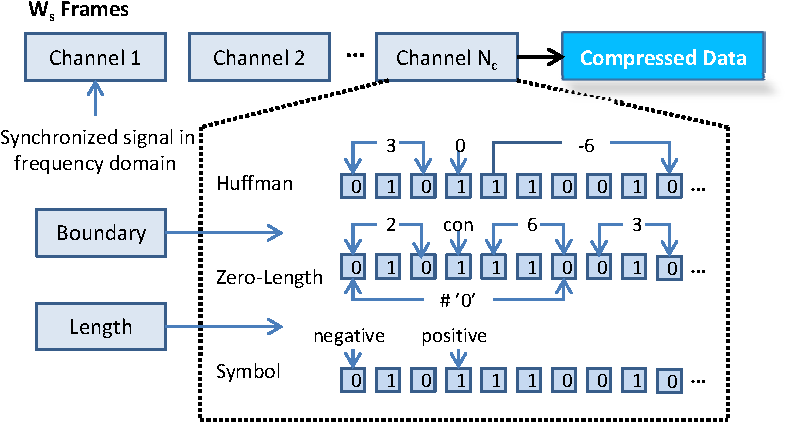
\includegraphics{Pictures/Compression/f8-crop.pdf}\\
  \caption{压缩数据格式化}\label{fig:Data Format}
\end{figure}





\section{实验}
这一节展现我们的实验结果,数据基于过去四年从两只猴子采集的数据。我们讨论了参数设定问题,并与经典信号压缩算法做了比较。

\subsection{数据集}

我们的实验数据及采集自浙江大学求是学院BMI系统 \cite{14}。为了训练猴子,建立了一套训练系统,该系统中,每只猴子在一个从中心出发的四方向摇杆上做训练,目标是根据可视的提示将方向杆摇至正确方向。完成了这项任务后,会对猴子大脑运动皮层(M1区)植入一个多电极阵列来捕捉手摇杆动作所产生的神经信号。每次试验持续大概60分钟。

这项任务在一个多通道捕获设备(Cerebus 128TM (Blackrock Microsystem, Salt Lake City, UT, USA))上完成,同时记录106个神经元的信号。 信号在96个电极(电极长1.0mm,总长度7.0cm)上进行采样,即以30kHz为采样频率,采96个通道,16-bit的分辨率。这样实验所获数据流为5.76MB/s, 也就每5分钟获得1.73GB的数据。为了检验我们的压缩算法,我们随机选择了12条记录,没条记录长300秒。




\subsection{评价标准}
为保证神经电信号压缩后的可用性,压缩算法在减少信息所占空间的同时希望保证重构信号的相对信息完整\cite{24}。从这个角度出发,我们需要一些压缩的评价标准来度量压缩效果。

\begin{enumerate}
\item{Signal to Noise Ratio}\\
在信息论中,信噪比(Signal to Noise Ratio, SNR)用来评判信号压缩的保真度。

令 $S_o$ 和 $S_r$ 分别表示原始信号和重建新号, SNR定义为$S_o$与$S_o-S_r$的能量比:


\begin{equation}\label{Eq:SNR Def}
  SNR(S_o,S_r)=10\cdot \log_{10} \frac{\left\|S_o\right\|_2^2}{\left\|S_o-S_r\right\|_2^2}
\end{equation}

作为一个基于能量的评判标准,SNR可以很好地反应误差的能量,但这还是不够的。回想我们在第\ref{sec:characteristic}节中分析的第一条信号特性,信号的主要能量集中在低频区域。也就是说低频区域对SNR影响很大,而这对高频区域就不平等了。为了解决这个不平等问题,我们将在另外的评判标准中聚焦于spike信号,也就是高频部分的主要有效信号。

\item{Spike ratio}\\
为了检验spike的保留程度,我们引入Spike Ratio, 表示一段信号与其压缩后重建新号相比保留的spike比例。在我们的验证中,常用的幅值阈值技术\cite{34}用来检测spike,其中阈值$Thr$设定为:


\begin{equation}\label{Eq: Spike Detection Threshold}
  Thr=\alpha \cdot \sigma_n,\ \sigma_n=median\left(\frac{|x|}{0.6745}\right)
\end{equation}

其中 $\alpha$ 是一个常量银子, $\sigma_n$ 是背景噪声的标准差估计量. 如果一个点的值大于 $Thr$,就视其为一个spike的起始点。 注意计算spike不留程度不是一个计数问题,而是计算匹配的spike个数,也就是有多少spike保留在了正确的位置。在此过程中,我们分别在原始信号和压缩重建新号上检测spike,并计算Spike Ratio。

为了帮助理解重建效果, 图\ref{fig:truncated_data}给出了一小段截取的数据在不同SNR和Spike Ratio上的压缩结果,其中黑线表示原始信号, 蓝色和绿色线表示重构信号,检测到的显著spike标注为下方的短线段。 图中(a). 蓝色线的重构效果: SNR = 31.02, Spike Ratio = 80\% (b). 绿色线的重构效果: SNR = 36.68, Spike Ratio = 100\%。 底部竖线段表示检测出spike的对应位置。


 可以看出,在右图中x=779处检测到的spike并未在左图中检测出来。这是因为信号在这里压缩时有一部分被丢掉了, 以至于在spike检测的时候没有达到式\ref{Eq: Spike Detection Threshold}中的阈值。 注意高SNR经常伴随着高Spike Ratio, 但也不一定总成立。因为SNR更多的反映了信号在低频能量上的特点。 


\begin{figure*}[htb]
  \centering
  % Requires \usepackage{graphicx}
  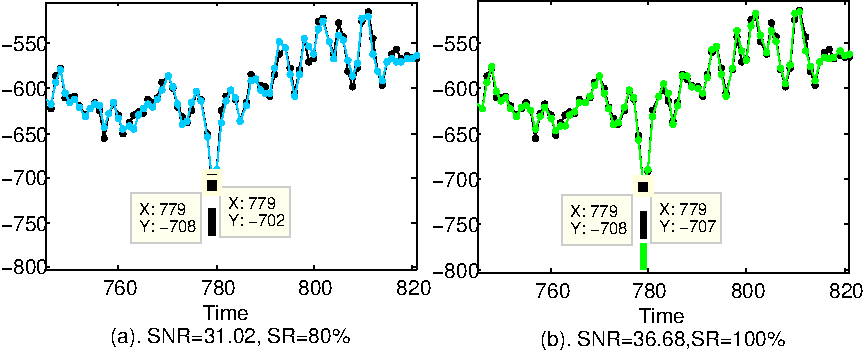
\includegraphics{Pictures/Compression/f9-crop.pdf}\\
  \caption{截断数据段的两个重构效果对比示意图。}\label{fig:truncated_data}
\end{figure*}


\item  Compression ratio
此外,我们还用压缩(Compression Ratio, CR)比来从数据冗余减少情况的角度度量压缩效果。压缩比定义为信号的压缩后大小除以原始信号所占空间。

\end{enumerate}

在下面的实验中,我们在以上三个评价标准上来衡量压缩算法的有效性。





\subsection{参数设置}
本小节中,我们讨论如何选定三个参数:  $T_{LH}$, 幅值过滤器的阈值; $\omega$, 量化表的比例; 和 $S_b$, 预处理中每个数据块的大小。


在我们提出的压缩框架中,有两个步骤会造成信息丢失:一是符号编码中的均值代替策略,而是高幅值分量的量化。这两个步骤都是在频域操作的,但是符号编码环节中,信息丢失最大为相应的量化表的值;而量化部分信息丢失最大为量化表对应值的一半。具体用哪一种方法进行压缩取决于高低幅值分量之间的界限,也就是取决于幅值滤波器的阈值$T_{LH}$。随着$T_{LH}$的升高,会有更多分量被符号编码压缩,带来更大的信号损耗而提高压缩率。因此,$T_{LH}$可以看做是重构效果和压缩比之间的协调系数。在我们的模拟中,$T_{LH}$在整个数据集上测试,以求的最佳的压缩效果。

另一个重要参数是量化表。为了在压缩过程中节省参数,量化表以LAC分量的平均幅值作为结果,在符号编码中进行共享。因此,QT会随着$T_{LH}$的增加而增加,从而在量化过程中可以粗化数据,降低其分辨率。 这里我们想了解能否通过调整QT的比例达到更好的压缩效果。 所以, 我们用QT乘以一个比例系数$\omega$来调整QT进行试验,其中,$\omega$在 $[0.5,2.5]$之间,以0.5为步长进行测试。


在不同参数下,我们的实验结果如图\ref{fig:Comparison-TLH}所示。 每个字图的横轴都是阈值 $T_{LH}$ . 不同大小的量化表用比例系数$\omega$表示, 其中 $\omega$ = 0.5(—), 1 (---), 1.5 (…), 2(-.-.-) and 2.5(-*-*-)。 每个子图的结果都是通过系统地调节阈值$T_{LH}$和比例系数$\omega$,然后在整个数据集上做结果的平均而来的。保持$\omega$不变,随着$T_{LH}$的上升,可以清楚地看到SNR和Spike Ratio都有所下降,这是因为高阈值会同时放大QT,相反这样会带来更优的压缩率。从图中可以看出,从SNR和Spike Ratio的角度来看,$\omega=1$ 的结果总是最优的;从Compression Ratio的角度来看,$\omega=1$的配置排在第二。容易理解为什么Compression Ratio随着$\omega$的增大而变化(降低), 因为$\omega$更意味着损失更多数据,导致Compression Ratio降下来。


\begin{figure*}[htb]
  \centering
  % Requires \usepackage{graphicx}
  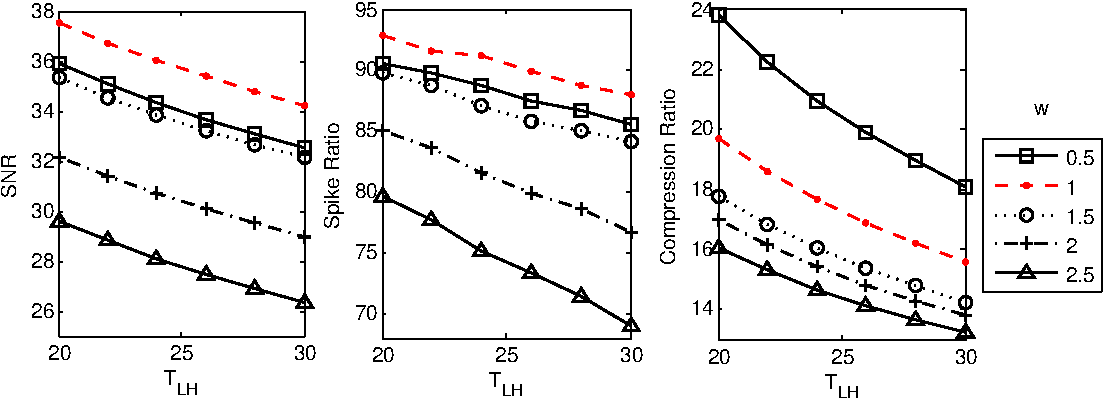
\includegraphics[scale=0.9]{Pictures/Compression/f10-crop.pdf}\\
  \caption{ 不同$T_{LH}$和QT下的 SNR, Spike Ratio 和 Compression Ratio。}\label{fig:Comparison-TLH}
\end{figure*}


图\ref{fig:Comparison-TLH} 展现了$\omega$是怎样影响压缩比和信号保真度的,但是由于没有一个$\omega$在3个评价指标上都达到最佳结果,所以我们仍然很难评判哪个$\omega$最好。 为此,图\ref{fig:Comparison:TLH-2}直观地表示出,在相同Compression Ratio的情况下,另外两个压缩评价标准的值。 该图是图\ref{fig:Comparison-TLH}的一个变换,图中横轴以压缩比作为自变量, 纵轴 (a). SNR, (b). Spike Ratio作为因变量, 每条曲线表示在不同QT的比例系数和阈值下的压缩效果。 可见,在相同Compression Ratio下$\omega=1$总是达到最好的效果。因此,对于无监督压缩,QT的比例系数为1时可以权衡压缩率和重构效果,给出一个理想的压缩结果。


\begin{figure*}[htb]
  \centering
  % Requires \usepackage{graphicx}
  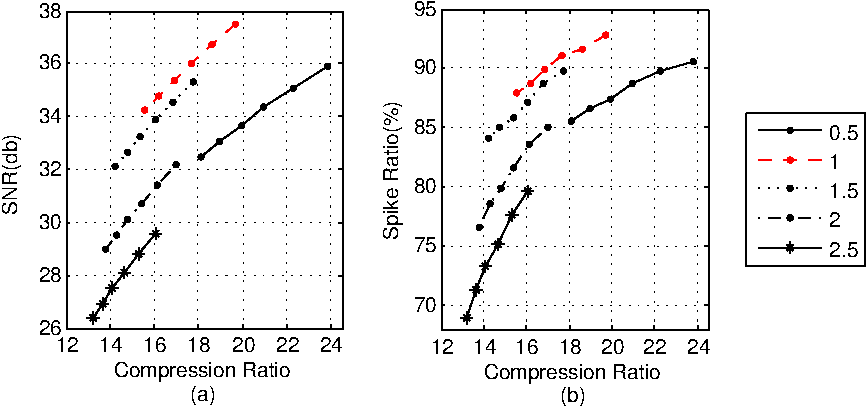
\includegraphics[scale=0.9]{Pictures/Compression/f11-crop.pdf}\\
  \caption{不同量化表比例系数下的压缩效果。 }\label{fig:Comparison:TLH-2}
\end{figure*}

$T_{LH}$的选择取决于我们的压缩要求。例如, 如果希望SNR大于30db且Spike Ratio不小于90\%的话,选择$T_{LH}=24$, 可以得到平均Compression Ratio为17.75\%, SNR达到36.24db, Spike Ratio大于90\%。 

最后需要确定的参数是预处理中的数据块大小$S_b$了。 在上述实验中,我们暂时都取$S_b = 1600$, 这里我们来讨论能否通过更改$S_b$达到更好的压缩效果。 实验结果如图\ref{fig:Comparison:Sb}所示, 其中横轴表示块大小$S_b$, 固定$T_{LH}=24$, $\omega$=1,  $S_b$ 在 1500 到 28500之间进行测试。


\begin{figure*}[htb]
  \centering
  % Requires \usepackage{graphicx}
  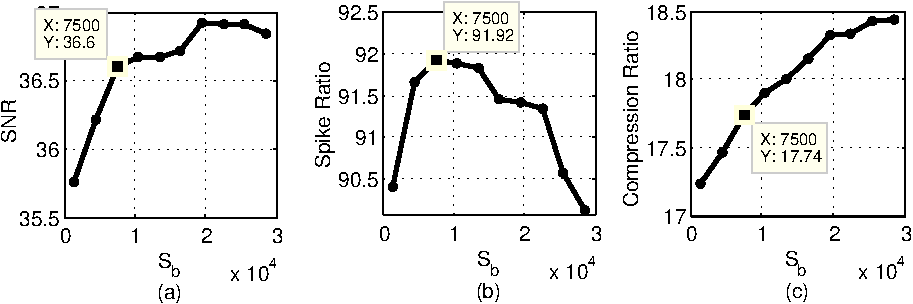
\includegraphics[scale = 1.1]{Pictures/Compression/f12-crop.pdf}\\
  \caption{不同块大小$S_b$下进行数据分割的压缩预处理的压缩结果。}\label{fig:Comparison:Sb}
\end{figure*}


该图说明随着$S_b$的增长,信号的保真度先提高后下降。原因如下:
首先,更大的$S_b$会使DCT系数更为精确,于是在IDCT(inverse DCT)的过程中降低误差。 但是, 这样会生成很多低幅值的DCT系数, 这样会使得归入LAC分量的值增多,也就是, 会有更多分量选用符号编码方法进行压缩, 这使得loss增大。 因此, 压缩保真度先增后减反映了上述两个因素之间的平衡。 根据给定的实验结果, 可以将数据块最佳大小设置为$S_b = 7500$, 这时达到整个数据集上平均Compression Ratio为17.7\%, SNR为36.6db, Spike Ratio为91.9\%。


\subsection{符号编码有效性}
在第\ref{sec:symbol_encoding}节中,我们提出了符号编码方法来压缩低幅值的DCT系数。 本节中给出实验结果, 探讨符号编码的有用性。 在上一节中我们已经选出最佳参数。 给定这些参数设置, 我们设计一个对比试验, 保持高幅值部分压缩方法不变, 对低幅值部分不采用符号编码而是整个丢弃, 以此来看符号编码所带来的改善。 比较结果如表格\ref{tab:T1}所示。\\


\begin{table}[ht]
\centering
  \begin{tabular}{c c c c}
  \hline\hline
  符号编码 & SNR(db) & SR & CR \\ [0.5ex] %insert table heading
  \hline
  有 & 31.4 & 83.7\% & 13.1\% \\
  无 & 36.6 & 91.9\% & 17.7\% \\
  \hline
  \end{tabular}
  \caption{SNR, Spike Ratio and Compression Ratio With and Without Symbol Encoding (Low-Amplitude)}
  \centering \label{tab:T1}
\end{table}


可以清楚地看出, 将低幅值分量考虑进来可以保存很多有效信息。 虽然这样会升高Compression Ratio, 但从SNR和Spike Ratio的角度来看,通过符号编码后重构效果有了很大提升。 这是由高频部分系数的内部分布决定的。 因此, 高频部分的符号编码是一个有效的压缩方法。



\subsection{方法比较}
由于在神经电信号压缩方面缺少统一的压缩标准作参照,而音频也是单维度时序信号, 所以我们在本节中选择与state-of-art的音频压缩算法作比较。 同时,我们也与其他传统数据压缩方法作比较。 通过与有损和无损压缩算法比较的试验结果可得,我们的压缩算法能够权衡重构效果和Compression Ratio。


\subsubsection{无损压缩}
本小节中讨论无损音频压缩和通用数据的压缩技术。无损压缩方法通过更为紧凑的编码格式对原文件进行编码, 使得数据编码后解压所得文件与原文件完全一样。 对音频压缩, FLAC之类的编码方法利用线性预测来估计信号频谱,可以对通用波形的Compression Ratio达到50\%到60\%\cite{23}。 但是神经信号不同于音频信号, 神经信号更为复杂,难以预测。 所以这类压缩方法即便用到神经信号压缩, 也不能获得较好的Compression Ratio。 类似的, 通用数据文件压缩方法, 如 Zip, 7-Zip 和 RAR 也不能达到相对较低的压缩率。 表\ref{tab:compression_ratio_comp} 显示出不同无损压缩技术的
压缩比。可见,在神经信号上最好的压缩方法是APE (Monkeys Audio), 得到最小压缩率为56.88\%。 注意,尽管神经信号被这些方法压缩后不能得到很好的压缩率, 但文件可以被完好的重建出来, 因此, SNR 是无穷大。 


\begin{table*}[ht]%开始表格
\caption{无损压缩方法性能比较} % 表格的名称
\label{tab:compression_ratio_comp} \centering
\begin{tabular}{|c||c|c|c|c|c|c|}%开始绘制表格
\hline
 & \multicolumn{5}{c|}{无损压缩编码} & Ours\\
  \hline \hline
 \multirow{2}{*}{类型} & \multicolumn{3}{c|}{音频编码} & \multicolumn{2}{c|}{文档文件格式} & SNR=36db\\
 \cline{2-6}
 & Lossless WMA & FLAC & APE & Zip & RAR &Spike Ratio=92\%\\
 \cline{1-7}
 压缩比 & 70.89\% & 54.27\% & 53.08\% & 70.04\% & 60.91\% & 17.74\%\\
\hline
\end{tabular}
\end{table*}



\subsubsection{有损压缩}
不同于无损压缩方法,有损音频压缩利用了人类听觉感应特点,即只对特定频率和幅值信号敏感,而丢弃其他对声音辨别率影响较小的琐碎信号。 所以音频的有损压缩只专注于量化病变吗那些容易感觉到差异的频谱部分。 本小节中以一个state-of-art的音频压缩方法(Advanced Audio Coding)为例, 与我们提出的压缩算法进行比较。 Advanced Audio Coding(AAC)是 MPEG-2 标准的一部分, 与MP3相比, AAC可以提供更好的信号质量, 同时将信号Compression Ratio多降低30\%。 图 \ref{fig:Comparison-AAC and Ours} 分别显示出这两种方法的 Compression ratio 对应重构效果。


\begin{figure}
  \centering
  % Requires \usepackage{graphicx}
  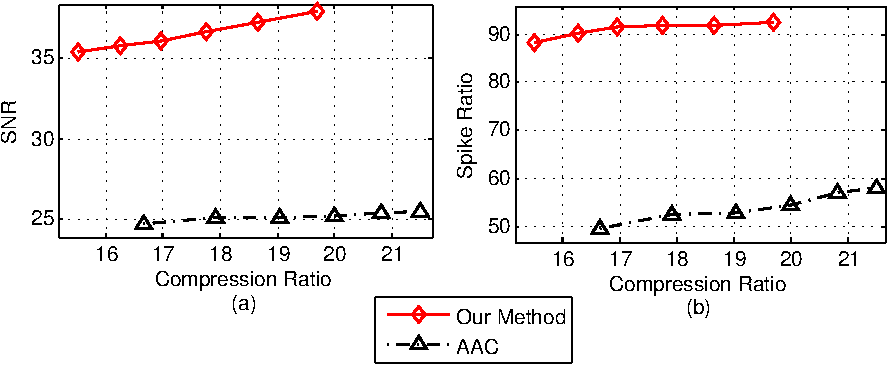
\includegraphics{Pictures/Compression/f13-crop.pdf}\\
  \caption{ 我们方法与音频编码方法压缩效果比较。 }\label{fig:Comparison-AAC and Ours}
\end{figure}


为了达到好的重构效果,我们对音频压缩选择高比特率,从 300kbps 到 600kbps。 

但是, 对于神经电信号,这两种方法的压缩效果并不理想。图中显示,在相同的压缩比下,我们的方法在两个信号保真度评判标准上都比AAC高, SNR超出AAC 46.4\%, Spike ratio超出AAC 80.4\%。 原因是音频压缩方法AAC在压缩过程中不关心哪部分对神经信号的处理比较重要。 实验结果也说明了神经电信号的信号特性有别于音频信号, 所以常规压缩方法不能很好地作用于神经电信号。 





\subsection{计算代价}
之前的小节描述了我们提出的算法在权衡Compression Ratio 和 重构误差时的有效性。 最后,我们讨论该算法的压缩效率。 一下结果是从我们在MATLAB上的实现中得来的统计结果。 初始化过程获取量化表, 哈夫曼码表和 无损压缩部分的分界线$B$ 速度为2.86Mb/s, 压缩过程为 0.13Mb/s, 解压速度为 0.14Mb/s。 如果用其他语言实现该算法压缩过程应该会得到更大提速。 




\section{结论}
本章提出了一个运动皮层神经电信号的压缩方法。 它在信号频谱采用提出的双阶编码方法进行信号压缩。 时序信号首先转换到频域, 然后通过一个幅值滤波器将信号分为 高幅值分量 和 低幅值分量, 然后分别对其进行编码。 为了压缩低幅值分量, 我们采用符号编码,对每个值只记录1bit的符号; 对于高幅值分量, 我们将其量化, 然后采用混合编码方法进行编码。 

之后, 我们将所提出的方法与其他压缩方法进行了比较。 可以看出, 在一定的Compression Ratio的情况下, 与其他方法相比, 我们的方法在重构效果(SNR 和 Spike Ratio)上都更胜一筹。 最终我们的压缩算法达到 17.7\% 的压缩比, SNR 为 36.6dB, 并保证91.9\%的 Spike 保真度。 该结果与其他神经信号压缩方法相比也很出众, 其他神经信号压缩方法只能使SNR达到 15-26dB, 压缩到元数据的1-20\%\cite{15,16,25}。 我们的算法在运动皮层(M1区)采集的神经电信号上进行了验证, 但是它也可以应用到其他神经信号上。 而且,如果考虑到其他信号的通道间相关性, 可以进一步提升压缩性能。 

而且, 基于统计结果而得的量化表,哈夫曼码表和其他参数可以根据信号被预先计算好。 我们的压缩框架原型成功地在猕猴运动皮层捕获信号上通过测试。 压缩效果比较理想, 只是有个缺陷, 本算法需要迭代求解, 因此比较耗时, 但由于压缩过程没有时序要求, 所以可在后期通过并行加速。














\chapter{卷积神经网络分析信号}
\section{深度学习介绍}

\subsection{传统机器学习方法与局限性}

在之前的50年左右,传统的模式识别模型用手工定义的特征进行特征提取,通过对数据的分析选取可训分类器进行模型构建。 最近10年,借助现代计算机计算能力的提高和大数据量的爆发,神经网络方法得以重新广泛应用,在很多领域都达到非常好的效果, 我们称这种利用大规模网络进行模式识别方法为深度学习(Deep Learning), 也叫End-To-End Learning。不同于传统模型采用固定特征,或者固定kernel(核函数)进行样本度量; 深度学习采用可训特征(或可训的kernel), 然后将特征作为可训练的分类器输入, 进行训练, 如表\ref{Tab:dl_overview_compare}。

\begin{table}[ht]
\centering
  \begin{tabular}{|c||c|c|c|}
  \hline
   & 特征 & 分类器 & 特点\\
  \hline\hline
   传统方法 & 人工定义的特征 & 简单可训练分类器 & 特征设计费时,需强业务背景\\
  \hline
  深度学习 & 训练特征提取模型 & 复杂可训练分类器 & End-to-End learning,feature易操作\\
  \hline
  \end{tabular}
  \caption{深度学习与传统模式识别方法}
  \centering \label{Tab:dl_overview_compare}
\end{table}

历史上,第一个有学习功能的机器为1960年提出的Perceptron\cite{rosenblatt1960perceptron},也是神经网络的一个基本单元。 Perceptron是一个简单特征提取器上加载的一个线性分类器: 


\begin{equation}
\label{Eq:Perceptron}
y=sign(\sum_{i=1}^N{w_iF_i(x)}+b)
\end{equation}


其中$x$为数据,$F_i(x)$为x的第i个特征,$w_i$为相应的特征权重参数, b为常参数, $sign$为分类器的非线性函数,对于二类分类,$sign$函数将结果映射到(0,1)。

\begin{figure*}[htb]
  \centering
  % Requires \usepackage{graphicx}
  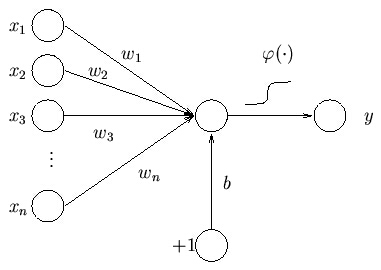
\includegraphics[scale=0.9]{Pictures/CNN/perceptron.jpg}\\
  \caption{Perceptront图例}\label{fig:perceptron}
\end{figure*}

目前最普及的实际应用也用到了线性分类器的一些变种,或者叫模板匹配(template matching)。 但是由于其底层的特征提取器需要反映特定信号的特点, 所以需要由特定领域专家来设置。 比如图像处理领域, 对于不同任务( 图像分类, 图像分割, 图像跟踪等), 所要求的特征就各不相同, 需要针对特定任务定义图像特征。 此外,传统方法也很难设计kernel, 从而不容易表达对距离的度量,仍然以图像来说,最简单的距离度量思路是对应像素相减,但是这显然不能表达图像语义层的相似信息。

为了能使特征更加灵活而且不过多依赖于专家指定的特征, 很多方法提出, 可以先人为定义简单特征, 然后通过无监督学习方法进一步得到中间层特征, 将其输入分类器进行最后分类。
典型的无监督特征学习方法如混合高斯模型\cite{jeong2004image,gray2001gauss,gauvain1992bayesian,reynolds2000speaker,reynolds1995robust, zivkovic2004improved,lee2005effective,yang1999gaussian}, K-Means\cite{liu2007computational,netzer2011reading,coates2011text,dy2004feature,coates2012learning}, 和Sparse Coding\cite{yang2009linear,boureau2008sparse,coates2011importance,coates2011analysis,gao2010local,mairal2010online}。 但这仍然不能解决以下几个问题:

\begin{enumerate}
	\item 建立传统模型代价大\\
	对每个领域,每个任务都需要设计特征。即便有了中间特征层进行无监督的特征选择, 庞大冗余的基础特征的设计也是耗时费力的。 随着工业界对不同任务的需求, 需要建立很多基础特征、 模型, 代价也很大。
	\item 无法很好地利用计算性能\\
	计算机性能的大幅提升本可以用来帮助加速机器学习, 但传统机器学习需要人工定义模型, 从而使模型规模受限,不能很好地利用计算性能和大量数据。 
	
	\item 人工定义特征效果欠佳\\
	目前, 自动学习的特征已经在图像、语音等很多领域强于人工定义的特征。 而且如果需要增加特征维度进行大规模学习就需要再手工定义更多特征, 而不能简单地够自动按比例扩大。
	
\end{enumerate}


\subsection{深度学习方法介绍}

深度学习是近几年来很热的机器学习算法, 在语音识别,计算机视觉,自然语言处理等领域打破了维持了多年的竞赛记录。以最典型的时序模型——语音识别的发展为例, 在1980年代早期, 主要应用Dynamic time Warping (DTW)\cite{juang1984hidden,myers1981comparative,rabiner1978considerations,berndt1994using}, 输入底层特征,通过无监督学习所得中间层特征输入分类器进行分类。 1985年后, \cite{huang1990hidden,rabiner1989tutorial,rabiner1986introduction}提出在中间层用隐马尔科夫模型描述一个序列出现的概率,得到进一步改进。 2010年左右, 使用深度神经网络进行逐层有监督学习达到最佳效果\cite{waibel1989modular,nakamura1989speaker}。


同传统方法的基本方法类似, 深度学习也是从数据分别生成底层特征, 中间层特征, 最后加入高层特征, 输入分类器进行分类, 即学习数据的结构化表示。 其形式化表示为:
\begin{equation}
y=f(W^kf(W^{k-1}f(...f(W^0X)...)))
\label{Eq:dl_formulation}
\end{equation}
其中, W为权重参数,k为层数,$W^iX$为输入X的线性表示, $f$为非线性函数, 如$tanh$ 函数。 深度学习就是优化$y$与groundtruth之间的距离,使之最小化。 从图像角度, 如图\ref{fig:feature_level}所示\cite{zeiler2014visualizing,zeiler2013stochastic},图中(a),(b),(c)分别为自动学得的底层特征,中层特征和高层特征, 其中底层特征学习图像的浅层特征,在所有类别中共享, 如(a)中,学到的特征类似Gabor滤波器所提取的边缘特征\cite{ngiam2010tiled,shi1998gabor}, 从中间层到高层依次学习图像更深层的语义特征, 如有语义的显著图像区域, 高层特征更为稳定,也具有类属性。  从自然语言处理的角度, 初始输入为字符, 从底层向上依次学习单词, 短语, 长句, 文章。

\begin{figure*}[htb]
  \centering
  % Requires \usepackage{graphicx}
  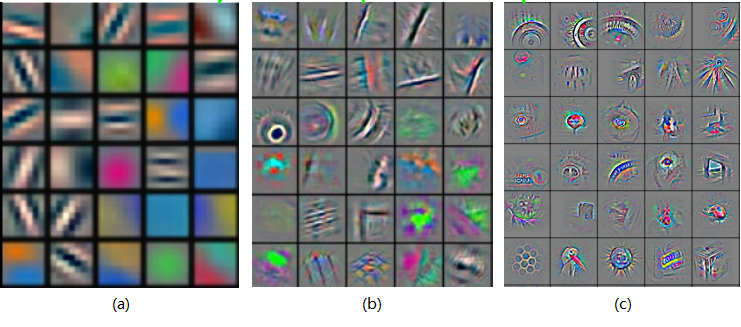
\includegraphics[scale=0.9]{Pictures/CNN/low_mid_high_feature.png}\\
  \caption{各层次feature}\label{fig:feature_level}
\end{figure*}


除了自动学习特征外, 深度学习和传统模型还有一个重要区别就是“深”。 一般来说, 深度结构由多层含参的非线性模型组成, 以形成特征的层次结构。
在\cite{bengio2007scaling,bengio2009learning}中讨论了深度模型的必要性。 浅层结构以现在的kernel machine\cite{scholkopf1999advances}为例, 如Support Vector Machine(SVMs)\cite{boser1992training,cortes1995support}。 这些方法定义特征
为一系列kernel函数连接而成的向量, 在训练数据中进行模板匹配, 如式\ref{Eq:kernel_fea_vec}所示。

\begin{equation}
	\label{Eq:kernel_fea_vec}
	\varphi(x) = [k(x,\mu_1),k(x,\mu_2),...,k(x,\mu_n)]
\end{equation}

式中, $\mu_i$为数据样本的一部分, 即模板样本; $\varphi(x)$为样本$x$的特征。 而后$\varphi(x)$通过线性组合进行分类:


\begin{equation}
	\label{Eq:kernel_predict}
	F(x) = W^T\varphi(x)
\end{equation}

可见, kernel方法就是一个简单的模板匹配层连接一个线性函数层, 由于方法中模板都是从原始训练数据中提取而得, 所以kernel machine的第一层
可视作一种简单的无监督方法, 只有式\ref{Eq:kernel_predict}中参数$W$的学习为有监督部分,没有涉及特征的层次结构, 因此不是深度模型。 同样,只有一个隐层的模型(如multilayer perceptron)也不算深度模型。 又如分类回归树(Classification and Regression Tree, CART), 其中所有决策都是在输入空间定义的, 同样没有根据特征的层次结构进行学习, 因此也不属于深度模型。 虽然有一些理论保证浅层结构可以很好地拟合任何复杂函数, 它们却无法保证特征的高效表征。 而深度模型可以从根本上通过简单设置网络结构更有效地表示特定函数。 最典型的深度结构就是有多个隐层的神经网络, 其中每个隐层节点之间的连接权重(如图\ref{fig:perceptron}中的$w_i$)都是通过有监督学习而来的, 因此可以很好地表征数据属性。



\begin{figure*}[htb]
  \centering
  % Requires \usepackage{graphicx}
  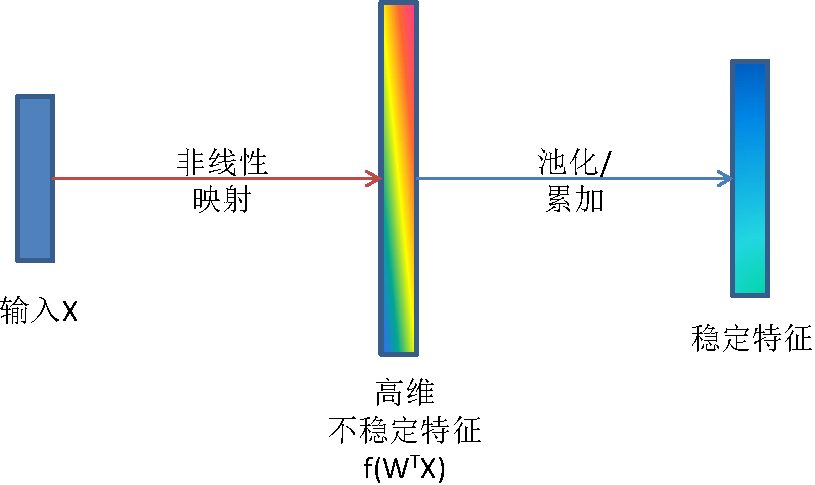
\includegraphics[scale=0.8]{Pictures/CNN/invariant-feature-crop.pdf}\\
  \caption{稳定特征生成方法}\label{fig:invariant_feature_learning}
\end{figure*}


神经网络在1940年代就开始了相关研究\citep{mcculloch1943logical,hebb1949organization}
, 但早期提出的神经网络多为线性回归的变种, 没有很大突破。 1965年, \cite{ivakhneko1995review}提出了第一个深度学习模型——Group Method of Data Handling (GMDH), 它通过回归方法进行网络训练, 再通过决策正则化去掉多余节点。 直到现在仍有很多应用以GMDH为基本框架, 如\cite{ikeda1976sequential,farlow1984self,madala1994inductive,kordik2003modified,witczak2006gmdh,
kondo2008multi}。 1960年代,受神经科学的启发, 神经网络也随之发展。 当时神经科学在猫的视觉皮层发现了简单细胞和复杂细胞, 简单细胞对特定视觉输入(如边缘的方向)敏感, 会做出一定响应; 而复杂细胞相对简单细胞表现出更为鲁棒的响应, 即不受空间变化的影响。 受此启发, 1979年 \cite{fukushima1979neural} 第一次在Neocognitron中引入了类似卷积神经网络的概念。 Neocognitron是为手写体识别提出的一个有层级结构的多层神经网络, 它不仅可以识别训练样本中的模式, 还可以识别训练样本经过平移, 旋转或其他变换后的模式。 其结构和现在我们用到的前向卷积神经网络比较相似, 层间连接也应用了现在我们常用卷积神经网络类似的部分权值共享(详见第\ref{sec:CNN}节)。 只是, Neocognitron通过无监督学习, 根据样本获得不同的pattern, 而不同于现在的有监督误差反传方法。 此外还有一些小差别,比如在pooling策略上, Neocognitron采用空间域平均, 而且虽然Neocognitron的层级较深, 但是它并没有在效果中考虑到深层带来的效果。 



由于90年代计算资源和数据量受限, 当隐层层数大于2的时候深度网络训练困难\cite{tesauro1992practical}, 所以之前神经网络的研究工作主要集中于浅层结构。 随着现在数据量的爆发, 神经网络的研究变得重新热门起来。 其基本思想是学习具有不变性的特征, 即,将输入数据映射到一个非线性的高维空间,使数据变得可分。 如\ref{fig:invariant_feature_learning}所示,输入经过非线性函数的映射到高维特征, 使数据变得可分, 但是这样的高维特征可能由于训练数据间差异导致不稳定,所以将高维数据中相似语义信息的成分通过池化(pooling)或累加等方法整合到一起, 形成稳定特征。





\subsection{深度神经网络结构与训练}

\begin{list}{•}
\item 网络结构\\
从网络结构来分, 神经网络有前向网络(包括multilayer neural nets\cite{kuurkova1992kolmogorov,
hornik1989multilayer,hornik1991approximation}和 convolutional nets \cite{lecun1995convolutional,krizhevsky2012imagenet},), 回馈网络(包括 stacked sparse coding\cite{yu2011learning}, deconvolutional nets\cite{zeiler2010deconvolutional})和双向网络(包括 deep boltzmann machines\cite{salakhutdinov2009deep,
srivastava2012multimodal,goodfellow2013multi}, stacked auto-encoder\cite{gehring2013extracting,vincent2010stacked,vincent2008extracting})三类\cite{lecun2013deep}。 目前, 前向网络使用最广, 如图\ref{fig:feed_forward}所示为一个前向网络的示意图。 

\begin{figure*}[htb]
  \centering
  % Requires \usepackage{graphicx}
  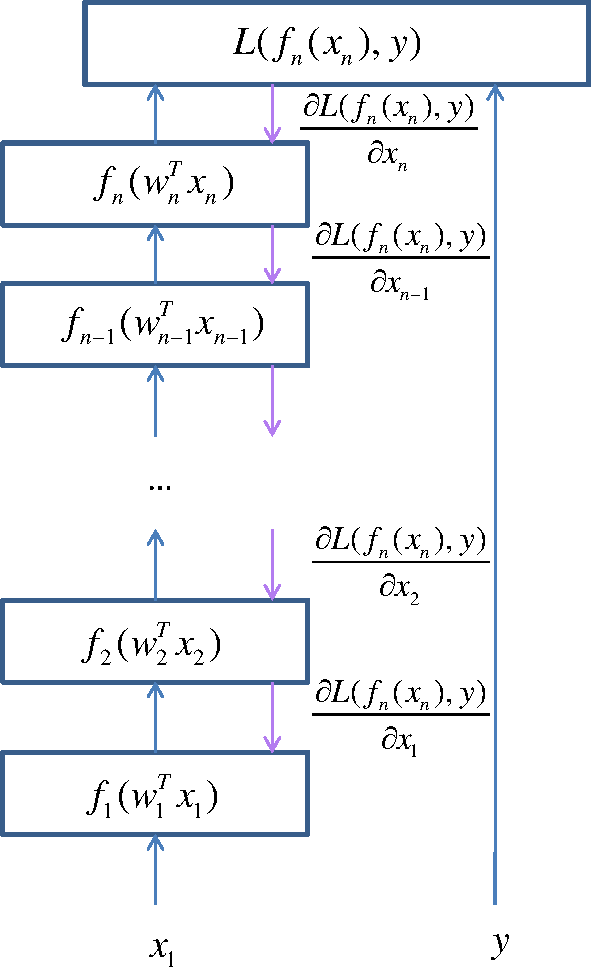
\includegraphics[scale=0.9]{Pictures/CNN/feed-forward-crop.pdf}\\
  \caption{前向网络的网络结构}\label{fig:feed_forward}
\end{figure*}

其中, $x_i$表示第i层的输入, 整个网络的输入为$x_1$; $w_i$表示第i层的参数, $w_i^Tx_i$得到$x_i$的线性组合; $f$为非线性函数, 每一层通过非线性函数将输入数据映射到下一层, 如图中蓝色箭头所示。 经过每一层非线性映射$f_i$的刀下一层输入,即
\begin{equation}
 x_i = f_{i-1}(w_{i-1}^Tx_{i-1})
\end{equation}

给定$x_1$对应的样本label$y$,我们的目标函数为$L(f_n(x_n),y)$, 其中$L$为损失函数。 常见的损失函数有平方损失, 指数损失, 对数损失等。 

\item 训练方法\\

自从1960年以来,不断有文章\cite{griewank2012documenta,director1969generalized,gray1965effect,bellman1962applied,
kelley1960cutting,bryson1961diffraction,}从变分法中的欧拉-拉格朗日方程出发讨论如何利用梯度下降(gradient descent, 也叫steepest descent)的方法\cite{hadamard1908memoire} 来进行神经网络中多层非线性可导函数的优化。
在这样的神经网络中, 可以通过链式法迭代地则对每个神经元求导\cite{bellman1962applied}。 之后,1970年, 误差反传算法(back-propagation algorithm, BP)\cite{hecht1989theory,goh1995back} 首次在Linnainmaa的硕士毕业论文\cite{linnainmaa1970representation}中提出, 其中描述, 误差反传算发可以高效应用于任意神经网络结构。 此后BP迅速应用到神经网络的训练中, 并实现了给定可导函数自动求解导数和BP\cite{speelpenning1980compiling}。 其基本思想如下: 由图\ref{fig:feed_forward}和式\ref{Eq:dl_formulation}可知, 在前向算法中从输入到输出经过了一系列非线性可导函数$f$的映射。 作为其逆过程, 如图中向下的紫色箭头所示, 在梯度下降算法的一步迭代中可用式\ref{Eq:bp_basic}计算参数$w_i$的变化。


\begin{align}
\label{Eq:bq_basic}
\frac{\partial L}{\partial w_i} 
&= \sum_t{\frac{\partial L}{\partial net_{i+1}}\cdot \frac{\partial net_{i+1}}{\partial w_i}}\\
&= \sum_t{\frac{\partial L}{\partial net_{i+1}}\cdot \frac{\partial w_{i+1}^Tx_{i+1}}{\partial w_i}}
\end{align}


其中, $net_k$为第k层输入$f$的线性组合,即


\begin{equation}
	net_k = w_k^Tx_k
\end{equation}


这样就可通过将误差逐层传递训练网络。 整个算法流程如算法\ref{algo:BP_basic}。


\renewcommand{\algorithmicrequire}{ \textbf{Input:}}      %Use Input in the format of Algorithm
\renewcommand{\algorithmicensure}{ \textbf{Output:}}     %UseOutput in the format of Algorithm
\begin{algorithm}
\caption{前向网络的误差反传算法}
\label{algo:BP_basic}
\begin{algorithmic}[1]  
\Require Data $x$, Label $y$
\Ensure  updated weight $w$
\For{k=K...1}
	\State \delta_t \leftarrow 0 \% signal variable
	\If{}
	\EndIf
\EndFor

\State	$k_z\leftarrow3,\varepsilon\leftarrow1$
\While{($\varepsilon=1$)}
    \For{$c\leftarrow1 to N_c$}
        \For{$i\leftarrow1 to S_b$}
            \State $\Omega_0(i)\leftarrow \sum_{c=1}^C 1_{\left\{H_c^Q[i]=0\right\}}$
        \EndFor
    \EndFor
    \State $T_{HZ}\leftarrow \frac{k_z}{k_z+1}$
    \State $x=CrossSegment\left(\Omega_0,T_{HZ}\cdot\frac{S_b}{N_s}\right)$
    \State $B=\left((x-1)+\frac{T_{HZ}\cdot \frac{S_b}{N_s}-\Omega_0(x-1)}{\Omega_0(x)-\Omega_0(x-1)}\right)\cdot \frac{S_b}{N_s}$
    \State $HCT\leftarrow Huffman Encoding(H_c^Q,B)$
    \If{($l_0(HCT)=\frac{3}{k_z}$)}
        \State $\varepsilon\leftarrow 0$
    \Else
    	\If{($l_0(HCT)\leq 3$)}
    	    \State $k_z\leftarrow \frac{3}{l_0(HCT)}$
    	\Else
	        \State $B\leftarrow 0,\ \varepsilon\leftarrow0$
	    \EndIf
    \EndIf
\EndWhile
\end{algorithmic} 
\end{algorithm}



\end{list}




在这三种为网络结构中, 卷积神经网络属于前向网络, 广泛应用于图像识别。 我们将在第\ref{sec:CNN}节中介绍卷积神经网络的结构与训练过程, 在第\ref{sec:cnn_configure}节中介绍我们的数据与网络配置, 最后在第\ref{sec:cnn_experiment}中给出实验结果。


\section{卷积神经网络}\label{sec:CNN}


\subsection{Perceptron}

\subsection{CNN网络结构}


\section{ConvP300Net}\label{sec:cnn_configure}

\subsection{任务描述}

\subsection{网络结构}

\section{实验结果}\label{sec:cnn_experiment}















%\chapter{卷积神经网络}



%
%
\section{插入图片}

论文中会插入图片\index{图片}、表格\index{表格}等元素。在Word中插图也是一件比较头疼的事,
涉及图的位置布置,大小,清晰度等问题。在\LaTeX 中这些问题也在一定程度上存在,
但\LaTeX 尽可能使得排版出来效果较好。相对于Word,虽然不是所见所得形式,
初期学习比较繁琐,但经短时间熟悉后可以比Word处理快不少。
我最喜欢的方式就是用Octave+gunplot把曲线图做成标准一样的大小,然后把这些图命好名,
放到一个专门的目录中去,一次全插好,如果要修改所有图的大小及式样,只要修改一下相应的Octave的生成曲线脚本文件即可。
这样整篇文档中的曲线图都是统一的模式,统一大小,统一字体,非常整齐。

下面对\LaTeX 中常见的插入图片方法作简要介绍,对于大部分专业做毕业论文应该是足够了,
更多更复杂的方式,有兴趣的可以查找相关专题说明文档\cite{epslatex},
这里提到的文献[\citenum{epslatex}]中给的是英文原版的下载地址,中文版搜一下网上到处有。

\LaTeX 支持的图片格式分两种情况:

\begin{enumerate}

\item{tex-$>$dvi-$>$pdf方式}

包括tex-$>$dvi-$>$ps-$>$pdf这样一个过程,本模版推荐采用的方式是tex-$>$dvi-$>$pdf,
这样的处理流程下,只能采用eps\index{eps}格式的图片。
如果你只有jpg\index{jpg},jpeg,png,gif之类格式的图片,那么不要紧,
\LaTeX 中提供了一个转换程序bmeps.exe\index{bmeps},可以帮助你把jpeg图片转换成eps格式,
当然你也可以用photoshop\index{photoshop},gimp转换。使用bmeps的命令格式如下:

bmeps -p 1 -c picture.jpeg picture.eps

其中,-p 1是压缩出的图片质量,1最好,2是默认,3最差。-c是保留彩色,不带c图片为黑白。

\item{tex-$>$pdf方式}

如果是用pdfTeX\index{pdfTeX}直接将tex转换为pdf的流程,则不能采用eps格式,但可以采用jpg,jpeg,
png,gif这些格式。

如果只有eps格式图片,则可以使用photoshop,gimp或者Acrobat\index{Acrobat}将其转为pdf格式。

这也是为什么这个模版带的文件中既有eps又有pdf的原因,
为了照顾到部分直接将tex转换到pdf的同学。

\end{enumerate}

{\bfseries 本模版推荐新手使用eps格式图片。}
eps格式没使用过\LaTeX 可能会比较陌生,eps也是一种矢量格式\index{矢量}图形。就是说如果是从矢量图形
转到eps格式,一样可以无损缩放。

subsection{图片插入的一般方法}

在文中插入图片的常用命令如下(以使用eps格式为例):

{
\linespread{1}
\zihao{-5}\noindent
\begin{verbatim}
\begin{figure}[htb]
\centering
\includegraphics{picture.eps}
\caption{图片标题}
\label{Figflag}
\end{figure}
\end{verbatim}
}

\verb+\begin{figure}[htb]+是告诉\LaTeX 软件准备插入图片,[htb]是一个选项,
代表图片的插入位置,h代表在文中当前位置,t代表一页的顶部,b代表页面底部,
还有一个选项是p,代表图片要单独放在一页中,如果不给出这些选项,
\LaTeX 会试着依次选用h-t-b-p方式,找出自已认为最合适的,如果给出一选项,
\LaTeX 就只使用给出的一个选项,如果给出几个选项,\LaTeX 会尝试给出的这几个选项,
然后选用它认为最合适的。
一般采用默认方式,不给出任何选项。除非有个把图\LaTeX 自动给出的位置不好,
再通过这几个选项来选择。

\verb+\centering+表示图片的位置为居中放置。

\verb+\includegraphics{picture.eps}+指出了要添加的图片的文件名,
如果图片在其它目录中,比如pictures文件夹,命令则变为:\\
\verb+\includegraphics{pictures/picture.eps}+。\\
要着重说明的是,插入的图片可以采用选项进行缩放\index{缩放},旋转。
比如,要把图片设置为同文字部分一样宽,如图 \ref{FigTextWidth} ,
则命令变为:\\
\verb+\includegraphics[width=\textwidth]{picture.eps}+

\begin{figure}[htb]
\centering

\includegraphics[width=\textwidth]{./Pictures/LHS.eps}
\caption{跟文字一样宽的图}
\label{FigTextWidth}
\end{figure}

指定为与文字一样宽太宽了,下面来把它缩小点,比如半个文字宽度,
那么就用\verb+width=0.5\textwidth+,如果指定10cm宽,就用width=10cm,
如果指定7cm高,就用height=7cm,如果是指定原图大小的50\%,就用
scale=0.5,如果我们想把它调整到原尺寸大小的50\%,再逆时针旋转90度
(如想顺时针旋转则使用负角度值),
就用如下的命令:\\
\verb+\includegraphics[scale=0.5,angle=90]{picture.eps}+\\
效果如图 \ref{FigHalfr90} 所示。

\begin{figure}[htb]
\centering

\includegraphics[scale=0.5,angle=90]{./Pictures/LHS.eps}
\caption{原图一半大小并逆时针旋转90度的图}
\label{FigHalfr90}
\end{figure}

常用的图片调整参数有:width,height,angle,scale这四个,
如果想要更多的效果,比如把图片四边裁掉,像Word中那样。
请参考graphicx\index{graphicx}包的帮助文件graphicx.pdf\footnote{此处要说明一下,
\LaTeX 安装的所有扩展包\index{扩展包}都有对应的说明文档,
请到\LaTeX 的安装目录中寻找,比如本模版使用的MiKTeX2.9的安装文件夹。
帮助文件文件名一般与扩展包名相同,格式为pdf或者dvi,少量的扩展包
帮助文件直接给的tex源文件,需要自行生成文档。}。

\verb+\caption{图片标题}+给出了图名,使用这条命令后,图下方就有了图名。
并且图片目录中也会出现相应的内容。如果图的名字比较长,有可能会造成图片
目录中的目录项换行,类似章节标题命令的格式,增加一个参数哪下:

\verb+\caption[图片目录中的标题]{图片下方出现的标题}+

\verb+\label{FigHalfr90}+这里给出了这个图片的标签“FigHalfr90”,
当你文档中要出现“如图 X.x所示”时,只要写成
“如图\verb+ \ref{相应的图片标签} +所示”即可。\LaTeX 会替你把标签换成图的编号。
这里要注意的是,一是引用命令前后各有一个空格,二是标签不能含有中文字符。

\verb+\end{figure}+表示图片插入结束。

这里提一些题外话,无兴趣研究\LaTeX 的同学请无视此段,
以上使用的图片插入命令并不符合\LaTeX 命令标准,
但是因为其方便应用,成为了应用最广泛的\LaTeX 命令。
标准的命令格式在graphicx.pdf中有详细说明。
另外,\LaTeX 还有一个图形扩展包,叫做graphics\index{graphics},注意最后一个字母,
一字之差,graphics包支持的功能更多一些,但大部分普通应用应用不到,
而且,graphics只支持标准命令调用。有兴趣的同学可以研究一下graphics.pdf,
此处我就不再多说了。

\subsection{插入图片的应用进阶}

刚才前面有提到:eps是一种矢量格式图形,所谓矢量格式图形,
就是放大缩小都会会造成图片变“糊”。其实,eps的方便之处还不止这些,
大部分的科学计算软件都支持生成eps格式图片,比如matlab,可以直接生成
eps格式图片。

有同学会说,那我用Microsoft Visio画的图怎么处理呢?Visio创建的图形也是矢量图,
在Word下是可以任意缩放的。如果你装有ps虚拟打印机或者acrobat,
这个问题就迎刃而解了。首先选中你要打印的visio图形,然后把它打印成ps或者pdf文档。
接下来ps文档的话就直接用安装CTeX组件时带的Ghostscrip转换成EPS图像,
pdf文档的话就先用Acrobat打开,菜单-工具-高级编辑-裁剪工具,
把所需要的图形那一部分剪出来,另存为eps文件即可。用photoshop同样可以达到这个效果。
这样出来的图像依然是矢量图,可以任意缩放不会糊。

\LaTeX 通过使用psfrag扩展功能包,还能对eps中的一些字符进行替换。
但是遗憾的是,psfrag只支持dvips转换程序,
本模版推荐使用的dvipdfm程序不支持该扩展包。
但这不要紧,我们可以采用变通的方法,把要替换字符的图用
tex-$>$dvi-$>$ps-$>$pdf的流程处理,
再生成的pdf用Acrobat裁剪后生成eps文件即可。

参考代码如下,生成图片效果对比如图 \ref{Figmatlab} 所示:

{
\linespread{1}
\zihao{-5}\noindent
\begin{verbatim}
\documentclass{article}
\usepackage{graphicx}
\usepackage{psfrag}
\begin{document}
\pagestyle{empty}
\psfrag{s1}{$y=sinx$}
\psfrag{x}{$x$}
\psfrag{y}{$y$}
\includegraphics{matlabfig.eps}
\end{document} 
\end{verbatim}
}

\begin{figure}
\centering
\includegraphics[scale=0.6]{./Pictures/matlabfig.eps}
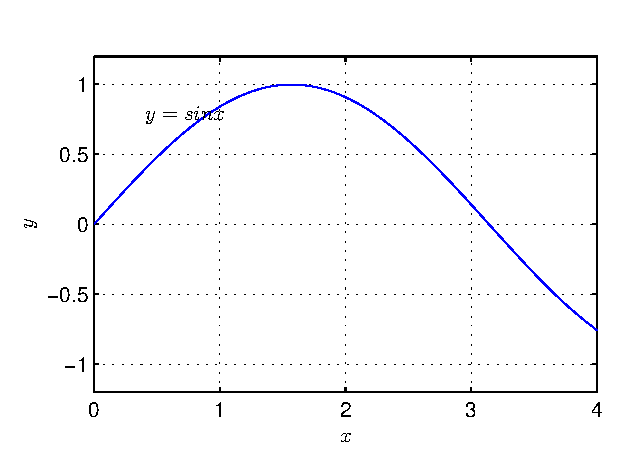
\includegraphics[scale=0.6]{./Pictures/matlabfigchg.eps}
\caption{matlab作图例}
\label{Figmatlab}
\end{figure}

图 \ref{Figmatlab} 中左图为matlab生成的eps图,右图为将左图中的s1,
纵横坐标名替换后的图片。可以把这一页放大几倍来看,图片依然非常清晰!
这就是矢量图的优势。
替换文字中如果有中文出现,因为dvips程序与cjk不兼容,
本论文模版的tex-dvi-pdf生成方式将不能用于含有dvips流程,使用dvips须使用cct方式,
具体请参考CTeX FAQ,有详细例子。

\section{插入表格}

\LaTeX 中建立表格比Word稍复杂一些,但表格的格式调整及效果比Word简单得多。

\subsection{普通表格的插入}

一个普通的插入表格代码如下所示,其生成的表格如表 \ref{Tabkeyword} 所示:

{
\linespread{1}
\zihao{-5}\noindent
\begin{verbatim}
{
\begin{table}[htb]
\zihao{5}
\caption{表格标题}
\label{Tabkeyword}
\centering
\begin{tabular}[t]{c|l|r|p{4cm}}
\hline
居中 & 靠左 & 靠右 & 靠左宽4cm\\
\hline
Center & Left & Right & Width=4cm\\
\hline
\end{tabular}
\end{table}
}
\end{verbatim}
}

\begin{table}[htb]
\zihao{5}
\caption{表格标题}
\label{Tabkeyword}
\centering
\begin{tabular}[t]{c|l|r|p{4cm}}
\hline
居中 & 靠左 & 靠右 & 靠左宽4cm\\
\hline
Center & Left & Right & Width=4cm\\
\hline
\end{tabular}
\end{table}

表格的使用一部分与图片相类似,比如开始的语句\verb+\begin{table}[htb]+,
以及结束的语句\verb+\end{table}+,与图片语句相比,除了把“figure”换成了
“table”,其它都相同。语句的含义也相同。

\verb+\zihao{5}+是把表格的字号改小一号,一般而言,表格字号应比正文字号小一号,
论文中的正文字号是小四号,那么表格中的字号就应该是五号字体。这个命令一定要写在
\verb+\begin{table}+ 的下方才能对该表格起作用。

\verb+\caption{表格标题}+是表格的标题,与图片标题格式相同,
会自动加到表格目录中去,如果表格标题太长,可以用
\verb+\caption[目录中的标题]{正文中的表格标题}+这种形式。

\verb+label{Tablekeyword}+与图片的标签相同,只要在正文中使用\\
\verb+\ref{Tablekeyword}+ 就可以在生成的文档中显示出表的编号,
同样,命令前后要各留一个空格,并且标签不能使用中文字符。

\verb+\centering+ 使整个表格居中放置。

\verb+\begin{tabular}[t]{c|l|r|p{4cm}}+是表格开始的标志,注意与
\verb+\begin+ \verb+{table}+区别开来,\verb+[t]+表示表格与其上方的正文行对齐方式是
行顶对齐,如果是\verb+[b]+则为行底对齐,这两种对齐方式可以在实际操作中试一下,
再做选择。\verb+{c|l|r|p{4cm}}+则代表这个表格各列的
对齐方式,c为居中,l为左对齐,r为右对齐,p\{4cm\}为该列宽度为4cm,并且左对齐。
中间接竖线“\verb+|+”则表示表格使用竖分隔线,如果没有这个竖线符号,对应位置就没有分隔线,
比如表 \ref{Tabkeyword} 就没有最左边和最右边的竖线。如果写为\verb+{|c|l|r|p{10cm}|}+,
就有最左边和最右边的竖线了。
如果不需要竖分隔线,则写为\verb+{clrp{10cm}}+
即可。要使用双竖线分隔线,就写为\verb+{c||c}+;还可以使用其它字条代替,
比如本模版的题名页中评阅人及答辩委员会信息就是利用的表格形式,它的分隔符是冒号“:”,
相应的命令就是\verb+{c@{:}c}+,即\verb+@{:}+。

\verb+\hline+就是画一条横线,如果没有写这一句命令,你会看到表格没有横分隔线。

表格内容是一行一行来填的,每一行结束使用断行符\verb+\\+,
同一行中不同列的元素用\&来分开。

\verb+\end{tabular}+表示表格结束。

\subsection{把表格换个样式}

上一小节介绍的方法生成的表格一般情况下可以用了,
但\LaTeX 的能力不止是做这样一个常规表格,
下面我们来利用booktabs-de\index{booktabs-de}扩展包来让表格看起来更professional一些。
这个扩展包的调用已经放在了本模版中了,使用本模版可以直接使用这种格式。
这个表格如表 \ref{Tab3Line} 所示。

{
\linespread{1}
\begin{table}[htb]
\zihao{5}
\caption{粗细线表格示例}
\label{Tab3Line}
\centering
\begin{tabular}[b]{cccc}
\toprule
长 & 宽 & 高 & 重量\\
(m) & (cm) & (mm) & (kg)\\
\toprule
1.234 & 5.676 & 332.876 & 3498.5\\
\midrule
548.4 & 23.43 & 34.98 & 923.8\\
\bottomrule
\end{tabular}
\end{table}
}

表 \ref{Tab3Line} 的实现代码如下所示:

{
\linespread{1}
\zihao{-5}\noindent
\begin{verbatim}
{
\linespread{1}
\begin{table}[htb]
\zihao{5}
\caption{粗细线表格示例}
\label{Tab3Line}
\centering
\begin{tabular}[b]{cccc}
\toprule
长 & 宽 & 高 & 重量\\
(m) & (cm) & (mm) & (kg)\\
\toprule
1.234 & 5.676 & 332.876 & 3498.5\\
\midrule
548.4 & 23.43 & 34.98 & 923.8\\
\bottomrule
\end{tabular}
\end{table}
}
\end{verbatim}
}

先解释一下这部分代码为什么会用一对大括号\{\}整个括起来。
如果要对文章中一部分内容的格式作调整,又不能影响到其它部分,
就使用一对大括号把要调整格式的部分括起来。
这里要调整的格式是行距。本论文的默认行距是1.5倍行距
\footnote{模版中的行距调整命令是$\backslash$linespread\{1.5\},
但并不是直接的1.5,这里有个换算,有兴趣的同学可以查看参考文献\cite{LaTeXshzh}},
在这里要把它调成单倍行距这个表格样式才比较美观,
因此就在最前使用\verb+\linespread{1}+命令把它的行距调整为单倍行距。
关于局部格式调整,在后面的《重点字符,醒目提醒》
一节中还将详细介绍,这里只对牵涉部分做简要说明。

这部分代码与普通表格代码的区别在于横线生成命令:\verb+\toprule+,\verb+\bottomrule+
都是比较粗的线条,\verb+\midrule+是比较细的线条。
此外,还有一个不完整线条命令,\verb+\cmidrule+,
该命令的使用类似下一小节要讲到的\verb+\cline+命令。

\subsection{有单元格合并的表格}

表格不可能总是一格归一格的。部分表格总是需要进行表格合并,
下面我就举一个表格合并的例子。\LaTeX 直接支持列合并,行合并则需要
扩展包multirow\index{multirow}的支持,本模版已经将该扩展包包含进去,可直接使用。
如表 \ref{TabComplex} 所示表格

\begin{table}[htp]
\zihao{5}
\caption{复杂表格示例}
\label{TabComplex}
\centering
\begin{tabular}[t]{|c|c|c|c|c|}
\hline
\multicolumn{2}{|c|}{我占了两列} & 第3列 & 第4列 & 第5列\\
\hline
\multirow{2}*{我占了两行} & 第二行第2列 & 第二行第3列 & \multicolumn{2}{|c|}{\multirow{2}*{我占了两行又两列}}\\
\cline{2-3}
& 第三行第2列 & 第三行第3列 & \multicolumn{2}{|c|}{} \\
\hline
\end{tabular}
\end{table}

表 \ref{TabComplex} 的实现代码如下:

{
\linespread{1}
\zihao{-5}\noindent
\begin{verbatim}
\begin{table}[htp]
\zihao{5}
\caption{复杂表格示例}
\label{TabComplex}
\centering
\begin{tabular}[t]{|c|c|c|c|c|}
\hline
\multicolumn{2}{|c|}{我占了两列} & 第3列 & 第4列 & 第5列\\
\hline
\multirow{2}*{我占了两行} & 第二行第2列 & 第二行第3列 & \multicolumn{2}{|c|}{\multirow{2}*{我占了两行又两列}}\\
\cline{2-3}
& 第三行第2列 & 第三行第3列 & \multicolumn{2}{|c|}{} \\
\hline
\end{tabular}
\end{table}
\end{verbatim}
}

\verb+\multicolumn{2}{|c|}{表格内容}+就是合并列的命令,参数2表示合并两列,
格式命令表示合并后的单元格居中对齐且两边有分隔竖线,注意在有分隔线时,分隔线符号
\verb+|+不要忘记。

\verb+\multirow{2}*{表格内容}+是合并行的命令,参数2表示合并两行,注意中间的*号。

注意同时合并行合并列时两个命令的嵌套方式,以及合并行情况下,除第一行外其它行的表示方式。
如合并两行两列时第二行的\verb+\multicolumn{2}{|c|}{}+。

\verb+\cline{2-3}+代表横线只划第二列与第三列,如果划2,3,5列,则写为\verb+\cline{2-3,5}+
\verb+\cmidrule+用法同\verb+\cline+。

\subsection{其它高级表格格式及扩展包简介}

如果需要实现表格左上角内有斜线的样式,
请使用slashbox\index{slashbox}扩展包并参考其自带帮助文档。

更复杂的表格,比如指定每一行的宽度,即可以借助盒子\cite{LaTeXshzh}来完成,
也可以借助扩展包array,tabularx等,具体实现代码此处不再详述,有兴趣的同学可参考文献
\cite{LaTeXshzh, Table:Lapo}以及扩展包内帮助文件。

\section{公式及其编号}

\LaTeX 出现之初的重要作用就是排版各种复杂的数学公式,关于数学公式的排版方法,
参考文献\cite{LaTeXshzh}中有一整章的内容来介绍各种公式的编辑。
我这里就偷个懒不写了,太长了,而且公式编辑我写不出我的特色来。

\LaTeX 的公式编辑效果远胜于Word中的公式编辑器,而且,使用LaTeX,
完全不用担心公式编辑器的版本问题,因为,这里公式就是用纯文本写的。
下面我举一个小小的公式例子来说明公式的编写及编号,如式 \ref{Equ:exm} 所示。

\begin{equation}
\label{Equ:exm}
c^2=a^2+b^2
\end{equation}

实现式 \ref{Equ:exm} 的代码如下所示:

{
\linespread{1}
\zihao{-5}\noindent
\begin{verbatim}
\begin{equation}
\label{Equ:exm}
c^2=a^2+b^2
\end{equation}
\end{verbatim}
}

\verb+\begin{equation}+与图片,表格很类似,开头都是一个环境开始命令,
只是这里的关键词是equation\index{equation}。

\verb+label{Equ:exm}+是给公式一个编号,以便在文中引用。该公式编号由\LaTeX 负责,
一般不需人工干预。

\verb+\ref{Equ:exm}+就是文中引用公式的命令。

\section{索引}

索引比较简单,只要在你想放索引的位置放上命令\\
\verb+\index{索引名}+,\\
然后文后面的索引列表中就出现“索引名”这个条目,并且有它的页码,
索引支持中文,英文字符。
如果文中有多处同名索引,这个表中都会把它们按字母表顺序列出来。
很方便的,你想在哪里插入索引就在哪里插入索引,完全不必考虑索引列表的事。

\section{参考文献}

前面介绍参考文献时就提到,只要准备好自己的参考文献数据库,
在引用参考文献时只需要利用\verb+\cite{tag}+就能把相应的参考文献引上。
这里的tag就是在参考文献数据库中各参考文献定义的标签,不能含有中文字符。
多个文献,则中间用英文逗号分开如\verb+\cite{tag1,tag2}+。
不需要考虑引用顺序,\LaTeX 会替你打理好一切。

如果想用形如“文献[1]提出XXX”的格式,则使用如下代码。

{\noindent\zihao{-5}\verb+文献[\citenum{tag}]提出+}

该模版已经把各类参考文献的列出格式按毕业论文要求调整好,不需要再修改。

如果你想了解更多参考文献格式调整的信息,请参考扩展包natbib\index{natbib},custom-bib\index{custom-bib}
自带的帮助文档。本次修订版新增的第5章也专门会对参考文献的格式校调问题进行大篇幅介绍。

\section{脚注}

有些时候需要使用脚注,\LaTeX 的脚注功能也是很方便的,
只要在你想要放一个脚注的地方用命令\verb+\footnote{脚注内容}+即可,
脚注内容长度不限,脚注编号\LaTeX 会替你操心。
你要做的,只是写好这个脚注的内容。

对于表格加脚注,就像表 \ref{ChapsecList} 显示效果那产,则稍显麻烦一点,需要把表格放进一个minipage里去。
关键代码如下:

{
\linespread{1}
\zihao{-5}\noindent
\begin{verbatim}
\begin{table}
……
\centering
\begin{minipage}[c]{10cm}
\centering
\begin{tabular}
……
\end{tabular}
\end{minipage}
……
\end{table}
\end{verbatim}
}

\verb+\begin{minipage}[c]{10cm}+表示创建一个内部居中对齐的,
宽度为10cm的小页面,这个宽度要根据其内部表格宽度来确定,
这样出来的脚注才美观。

\section{重点字符,醒目标示}

有的时候需要对某些内容做一个醒目标示,比如改变字体啦,字体加粗啦。
这个时候首先要把需要改变格式的部分用一对大括号
\footnote{要使用英文字符的大括号\{\}}括起来。
然后在头上写上字体字号之类的命令。就像这样

我这一段话里有{\bfseries 加粗},
{\kaishu\bfseries 有楷体并加粗},有{\heiti 黑体},还有{\zihao{3}三号字}字体。

这一句话的实现代码如下:

{
\linespread{1}
\zihao{-5}\noindent
\verb+我这一段话里有{\bfseries 加粗},{\kaishu\bfseries 有楷体并加粗},有{\heiti 黑体},还有{\zihao{3}三号字}字体。+
}

在\LaTeX 中可以用的字体有{\songti 宋体}\verb+\songti+,{\fangsong 仿宋}\verb+\fangsong+,
{\kaishu 楷体}\verb+\kaishu+,{\heiti 黑体}\verb+\heiti+,
{\youyuan 幼圆}\verb+\youyuan+,{\lishu 隶书}\verb+\lishu+六种。字号命令是\verb+\zihao{1}+字号从
1,-1,2,-2,一直到8号字,前面带负号表示小号字,比如-4就是小四号字体。
7,8两个字号没有小号字对应。

关于加粗字体命令\verb+\bfseries+,对英文字符只要使用\verb+\bf+即可,
中文字符应使用\verb+\bfseries+。

关于字体效果的设置,更多内容参见CTeX自带的帮助文档ctex.pdf。

如果想使用更多的字体,比如微软雅黑,请自行网络搜索方法,自己生成字体文件并关联上即可。
CTeX提供的六种字体,一般情况下已经足够使用。



%
%\section{插入算法伪代码}
%以下是插入算法伪代码示例,如算法\ref{alg:skeleton_dt}所示。
%
%\begin{algorithm}[!htb]
%\caption{基于距离变换的骨架提取}
%\label{alg:skeleton_dt}
%\begin{algorithmic}[1]
%\Require 前景的二值图 bw \Comment{像素的灰度值为0或1} 
%\Ensure 骨架图 skel
%\State // 第1次遍历:从上往下,从左往右
%\For{$i=1,\dots ,M$} \Comment{M是二值图的高度}
%    \For{$j=1,\dots ,N$} \Comment{N是二值图的宽度}
%        \State bw[i][j] = 1 + min(bw[i][j-1], bw[i-1][j])  \Comment{min函数取极小值} 
%    \EndFor
%\EndFor
%\State // 第2次遍历:从下往上,从右往左
%\For{$i=M,\dots ,1$}
%    \For{$j=N,\dots ,1$}
%        \State bw[i][j] = 1 + min(bw[i][j], bw[i+1][j], bw[i][j+1])
%    \EndFor
%\EndFor
%\State // 第3次遍历:获取骨架图
%\State skel 的空间分配,并将每个像素初始化为0
%\For{$i=1,\dots ,M$}
%    \For{$j=1,\dots ,N$}
%        \State t = max(bw[i-1][j], bw[i+1][j], bw[i][j-1], bw[i][j+1])  \Comment{max函数取极大值} 
%        \State t = max(t, bw[i-1][j-1],bw[i-1][j+1],bw[i+1][j-1],bw[i+1][j+1])
%        \If {bw[i][j]>=t}
%        	\State skel[i][j]=1 \Comment{骨架点} 
%        \Else 
%        	\State skel[i][j]=0
%        \EndIf
%    \EndFor
%\EndFor
%\end{algorithmic}
%\end{algorithm}
%
%\section{插入源代码}
%代码示例:
%
%\begin{lstlisting}[language=C] 
%int main(int argc, char ** argv) 
%{ 
%	printf("Hello world! \n"); 
%	return 0; 
%} 
%\end{lstlisting} 
%
%\section{插入定义、定理等}
%实例来自 https://github.com/eclipselu/zjuthesis-mphil。
%
%\begin{hypo}
%待月西厢下,迎风户半开;隔墙花影动,疑是玉人来。
%\begin{eqnarray}
%  \label{eq:eqnxmp}
%  c & = & a^2 - b^2\\
%    & = & (a+b)(a-b)
%\end{eqnarray}
%\end{hypo}
%
%\begin{defin}
%子曰:「道千乘之国,敬事而信,节用而爱人,使民以时。」
%\end{defin}
%
%\begin{theo}
%犯我强汉者,虽远必诛。\hfill —— 陈汤(汉)
%\end{theo}
%
%\begin{pro}
%天不言自高,水不言自流。
%\begin{gather*}
%\begin{split} 
%\varphi(x,z)
%&=z-\gamma_{10}x-\gamma_{mn}x^mz^n\\
%&=z-Mr^{-1}x-Mr^{-(m+n)}x^mz^n
%\end{split}\\[6pt]
%\begin{align} \zeta^0&=(\xi^0)^2,\\
%\zeta^1 &=\xi^0\xi^1,\\
%\zeta^2 &=(\xi^1)^2,
%\end{align}
%\end{gather*}
%\end{pro}
%


\chapter{基于循环神经网络的信号解码}

\section{循环神经网络(RNN)}

人类可以很快地识别节奏模式序列,即那些有时间间隔的子模式。此外,鼓手等演奏者也能根据运动命令生成有精确时间节奏的节奏序列。这促使人们研究人工系统,去分离或产生通过事件间时间间隔长度传递信息的模式。

Deep Neural Network(DNN)通常在较难的learning问题上能够达到比较好的效果。在实际问题中有很多是时序信号,如语音识别, 连续(即字符无分割的)手写识别, 蛋白质分析,股市预测等。虽然这些问题无论是否有监督,都可以交给CNN或者DNN处理并达到较好效果\cite{abdel2014convolutional,lecun1995convolutional,ciresan2011convolutional,lecun1994word ,lauer2007trainable,baldi1996hybrid,zhu2014stock},但是并不能完全利用上信号的时序性,而循环神经网络(recurrent neural network)可以利用神经元循环传递实现时序信号的分析。

一个循环神经网络是一个结构中带反馈连接的神经网络,它可以学习并处理时序序列问题,而传统的机器学习算法由于没有考虑时间方面相关性可能并不善于解决这类问题。之前对于这种时序信号的处理方法是一些基于可学习可适应的方法,如隐马尔可夫模型\cite{eddy1996hidden},前向网络等,但是在计算能力和物理意义上RNN都比这些方法能力强。而且事件在时域上的信息很大程度上反映了时序任务的重要信息,如运动控制和节奏检测。隐马尔可夫模型往往忽视这一信息,而循环神经网络( Recurrent Neural Network, RNNs)可以从根本上学习应用这个信息。隐马尔可夫模型(HMM)能够成功地应用在语音识别,正是因为这种方法不喜欢特定口语单词语速产生的差异。而如节奏检测,音乐处理,和其他本文中所述的任务,都需要精确的时间测量。虽然HMM可以通过给每个时间间隔单独创建一个内部状态来解决有限个时间间隔的问题,但是这样既麻烦又低效的,并且没有用到HMM的非线性时序伸展不变性。

事实上,尽管隐马尔克夫模型和传统的离散符号语法学习设备被限制在离散状态空间, RNNs在根本上上适用于所有的序列学习任务,因为它们具有图灵能力\cite{siegelmann1995computational}。典型的RNN学习算法在一个潜在抗噪算法的通用空间中进行梯度下降\cite{pearlmutter1995gradient},这个通用算法采用分布式,用连续值表示的内部状态来将实值的输入序列映射为实值输出序列。所以循环神经网络在识别由时间距离定义的模式上更有希望。混合HMM的RNN方法\cite{bengio1995input}可能能够结合两种方法的优点,但就我们所知,从未被用到准确的事件计时的问题。

然而,Schmidhuber的学生Hochreiter在他的博士论文\cite{hochreiter1991untersuchungen}中指出了RNN的缺点:vanishing or exploding gradients:
在传统RNN中,反传的误差要不就收缩太快,要不就爆发超出界限。事实上误差会随着网络层数而指数型衰减或爆发,因此很难训练, 而且不能处理长时间延时事件。

之后Hochereiter提出了一种新型的RNN——长短时间记忆Long Short-Term Memory \cite{hochreiter1997long},它在涉及很长一段时间延时的任务上比传统RNNs更好。LSTM网络中的基本单元是包含一个或多个存储单元(memory cell)和所有cell共享的三个自适应乘法门(图2)的存储块(memory block)。每个存储单元都在其中心有一个自连接单元,我们称之为“恒误差旋转木马”( Constant Error Carousel, CEC ),它本质上是一个无参数的线性单元。通过无限循环地进行激活和误差信号传递,CEC可以在延长的时间段内提供短期存储。Gers et al在LSTM中安置了忘记门 \cite{gers2000learning}。输入,忘记和输出门可以通过训练分别进行学习,即学会将什么信息存入,怎样保存,什么时候读出。

 

LSTM的体系结构允许LSTM容忍输入的事件之间有很长的时间延时(1000步及以上);而传统RNN用代价更高的更新算法,比如BPTT \cite{williams1990efficient},RTRL \cite{robinson1987utility,williams1989learning},或它们的组合\cite{schmidhuber1992fixed,williams1995gradient},都无法学习超过10个时间延时的序列\cite{hochreiter1991untersuchungen,bengio1994learning,hochreiter1997long, gers2000learning,hochreiter2001gradient}.

比如,一些我们以前任务需要用LSTM网络对发生于50个离散时间间隔之前的事件予以响应,而不受发生于之前49个时间间隔的事件的影响。就在关键时刻之前,如果有一个有用的“标记”输入通知网络,其下一步的行动将是至关重要的。因此,网络没有必要学习度量50个步骤的时间间隔;它只需要学会保存这50步的相关信息,而后一旦观察到这个标记就用这段信息即可。

但是如果没有这样的标记呢?如果网络本身需要学习测量并在内部表示这段特定任务的间隔内信息,或生成由特定时间间隔分割的序列模式,就要求在长时间连续输入流中保持网络的时间精确行和鲁棒性。显然,这样的任务通常不能由基于共同时间窗口的方法解决的,因为它们的泛化能力受时间窗口大小的限制。不幸的是,这意味着我们不能用标准基准进行测试和计时,因为就我们所知,目前没有任何其他网络学会将15个时间滞后推广到45个等。因此,我们不得不以创建一组新的比较任务。那就将用到LSTM了。

因为长短期记忆方法已被证明在长时间滞后任务上比其他RNN的方法强,而且其体系结构与人脑对信息的处理方式很类似,考虑到这种方式可能可以更好地模拟大脑皮层信号激发方式,所以我们研究该方法。LSTM通过内部细胞到多门的“窥孔连接”,在没有任何段式训练样本的情况下可以很好的区分50个和49个时间间隔的spike序列。在没有外部复位和监督学习的情况下,LSTM的变种也能学习生成时间精确的稳定spike流和其他非线性周期模式。这使得LSTM在需要的精确测量或生成有时间间隔的任务上很有效。






\section{LSTM的应用}

我们先来看一下LSTM的已有应用:

\begin{enumerate}
\item{语音识别}
LSTM RNN是著名语音识别数据库TIMIT的benchmark (Graves et al, ICASSP 2013),Nicole等人用LSTM网络进行RNN的retraining\cite{beringer2005classifying},这是无法在HMM中实现的。google用LSTM RNN来改善大规模语音识别\cite{sak2014long}。在类似问题上,\cite{sutskever2014sequence}将LSTM应用在机器翻译问题,实现了sequences to sequence学习。



\item{连续(即字符无分割的)手写识别}
Connectionist Temporal Classification(CTC)\cite{graves2012connectionist}训练的RNN(CTC-LSTM)\cite{bluche2014a2ia},在2009年跑得结果赢了很多手写识别竞赛的冠军\cite{graves2006connectionist}。



\item{音乐合成}
通过训练,RNN的变种RNN-RBM可以无监督地形成简单的钢琴旋律。[5] Modeling Temporal Dependencies in High-Dimensional Sequences: Application to Polyphonic Music Generation and Transcription.通过用音乐集训练LSTM网络,网络就可以无监督地生成有特定样式的旋律与和弦的音乐样本。而前向网络和传统RNN都无法学习出和弦音。\cite{eck2002first}



\item{蛋白质分析}
在RNN中还可以实现无分割的蛋白质分析\cite{hochreiter2007fast},其本质和无分割的手写体识别同理。

\end{enumerate}






\section{循环神经网络网络结构}
\subsection{RNN网络结构}

首先我们来看RNN的结构:
RNN包含一些用带权连接的单元,每个单元有一个在时间$t$更新的激活函数$y(t), t=1,2,…$。对单元$i$的激活$y^{i}$通过计算网络中与$i$的相连输入$net^{l}(t)$得到:
\begin{equation}
	net^{l}(t) = \sum_m{w_{im}y^m(t-1)}
\end{equation}
而后通过一个可导函数$f$将$net^{l}(t)$进行”压平”($f$比如我们之前提到的sigmoid, tanh, 或Relu函数):
\begin{equation}
	y^{i}(t) = f(net^i(t))
\end{equation}
其中网络的输入是随时间变化的序列,对于传统的RNN回归问题或者序列分类问题(如手写体识别),输出也是随时间变化的序列。而对于纯分类问题,输出只是一个标量。为了方便讲述传统RNN的方法,我们在这里使用输入输出都是时间序列来描述。

对有监督的RNN而言,当采用平方和误差作为loss时,我们将每个单元的损失计为与其输入与真实输入之差,而全局损失函数为所有样本损失的平方和,即t时刻的总误差为:
\begin{equation}
 \begin{array}{lr}
E(t) = \frac{1}{2}\sum_i{{e_i(t)}^2}\\
e_i(t) := Y^i(t) –y^k(t)
 \end{array}
\end{equation}

整个序列的误差为每一时刻的误差$E(t)$之和。


和CNN类似,RNN可以用梯度下降进行网络参数更新,即对于每个权重$w_{im}$,有
$\partial w_{im} = -\alpha \frac{\partial E(t)}{\partial w_{im}}$,其中$\alpha$为学习率。这种方法也是标准RNN的更新方法backpropagation through time (BPTT)方法,通过带入可得t时刻i单元的误差信息为

\begin{equation}
\partial e_i(t) = f_i’(net_i(t))\sum_j{w_{ji}e_j(t+1)}
\end{equation}

然而在1990年,Schmidhuber的学生Hochreiter提出RNN在理论上很好,但是不好训练,误差会以指数增长或者消失\cite{williams1995gradient},原因是BPTT, real-time recurrent learning(RTRL)\cite{williams1989learning},这类基于梯度下降的方法都有一个问题,如果计算权重更新后的q步,则如公式\ref{Eq:rnn_bptt}所示,t时刻与t-q的更新误差之比与$w_{lv}$有关,

\begin{equation}\label{Eq:rnn_bptt}
	\frac{\partial e_v(t-q)}{\partial e_u(t)} = 
	\left\{
	\begin{array}{lr}
		f'v(net_v(t-1))w_{uv}, q=1\\
		f'v(net_v(t-q))\sum_{l=1}^n{\frac{\partial e_l(t-q+l)}{\partial e_u(t)}w_{lv}}, q>1
	\end{array}
	\right.
\end{equation}

将上式$q>1$的情况展开,用$l_t$表示t时刻的该节点,$l_q = v, l_0 = u$,可得:
\begin{equation}
 \frac{\partial e_v(t-q)}{\partial e_u(t)} = \sum_{l1=1}^n ... \sum_{m=1}^q{\prod_{m=1}^q{f_{l_m}'(net_{l_m}(t-m))w_{l_ml_{m-1}}}}
\end{equation}

其中$\prod_{m=1}^q{f_{l_m}'(net_{l_m}(t-m))w_{l_ml_{m-1}}}$决定了总的传回误差。所以如果$|{f_{l_m}'(net_{l_m}(t-m))w_{l_ml_{m-1}}}|>1.0$,,则最大的乘积随q指数增长,就会使学习过程不稳定;相反地,如果$|{f_{l_m}'(net_{l_m}(t-m))w_{l_ml_{m-1}}}|<1.0$,则最大的乘积随q指数下降以至消失,在有限时间内无法学到有效网络参数,这也被称为长时间延时问题(long time lag problem),使得RNN的应用一度局限在短时间序列,而我们在绪论中提到的长短时间记忆方法有效克服了这一问题,我们将在下一节中予以介绍,关于RNN,更多优化方法请参考Bengio在\cite{bengio2013advances}中的综述。





\subsection{LSTM的网络结构}
LSTM通过设置恒定的传递误差来解决上面提到的问题。在基本LSTM单元中,LSTM引入了一个自连接线性单元,称作误差旋转木马(error carousel), 恒定的传递误差中设定权重$w$恒等于1,$f$为线性函数,目的是这各部分只起到传递误差的作用,而将学习参数作用于其他权重。

粗略地表示,我们在第一章中简单介绍了LSTM。它以memory block作为基本单元,其中包含一个至多个memory cell,典型的LSTMmemory cell如图\ref{Fig:lstm_simple}所示:
核心有一个线性单元(或者称作线性神经元,如图橘黄色所示),这是个线性单元,在任意给定时间,该单元将其所有输入通过加权连接求和。它的自循环连接权重固定为1(即与左边紫色圆点之间的半圆连接权重固定为1),这样通过确保训练信号或者误差在被传递的时候不会消失(vanish)克服了原先RNN的一个主要问题:vanish(参考3.2节)。而且这个核心神经元为线性让LSTM实现了可以识别多达1000步之前的模式。


\begin{figure}[htb]
  \centering
  % Requires \usepackage{graphicx}
  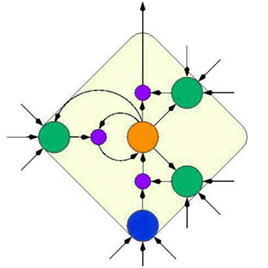
\includegraphics{Pictures/LSTM/lstm_simple.png}\\
  \caption{LSTM模型}\label{Fig:lstm_simple}
\end{figure}

在这个核心周围是非线性可适应神经元,用来学习非线性神经动作。图中蓝色神经元用来表示输入,三个绿色神经元分别表示三个门(左边的是忘记门,右下角为输入门,右上角为输出门),这些门通过学习来使核心线性神经元不受无关事件和误差信号的干扰,而又能通过有效信息更新网络参数,即门是否打开来决定信号的有效性。最后,紫色圆点用以表示乘积操作。LSTM的学习算法是非常高效的,每个边权的计算复杂度不超过O(1)。


LSTM的应用中,可以将多个memory cell进行组合,如图\ref{Fig:lstm_mixture}所示混合模型。其中有两个memory cell,分别从输入和输入门接受输入,每个cell将输出结果分别传给另一个memory cell的输入, 输入门, 输出门和忘记门。 但实际应用中,通常将一至多个memory cell组合成memory block,共享输入,输出,忘记门的权重(而不共享输入的权重),这样可以减少自适应参数的数量,同时使block内部各cell起到不同作用。 

\begin{figure}[htb]
  \centering
  % Requires \usepackage{graphicx}
  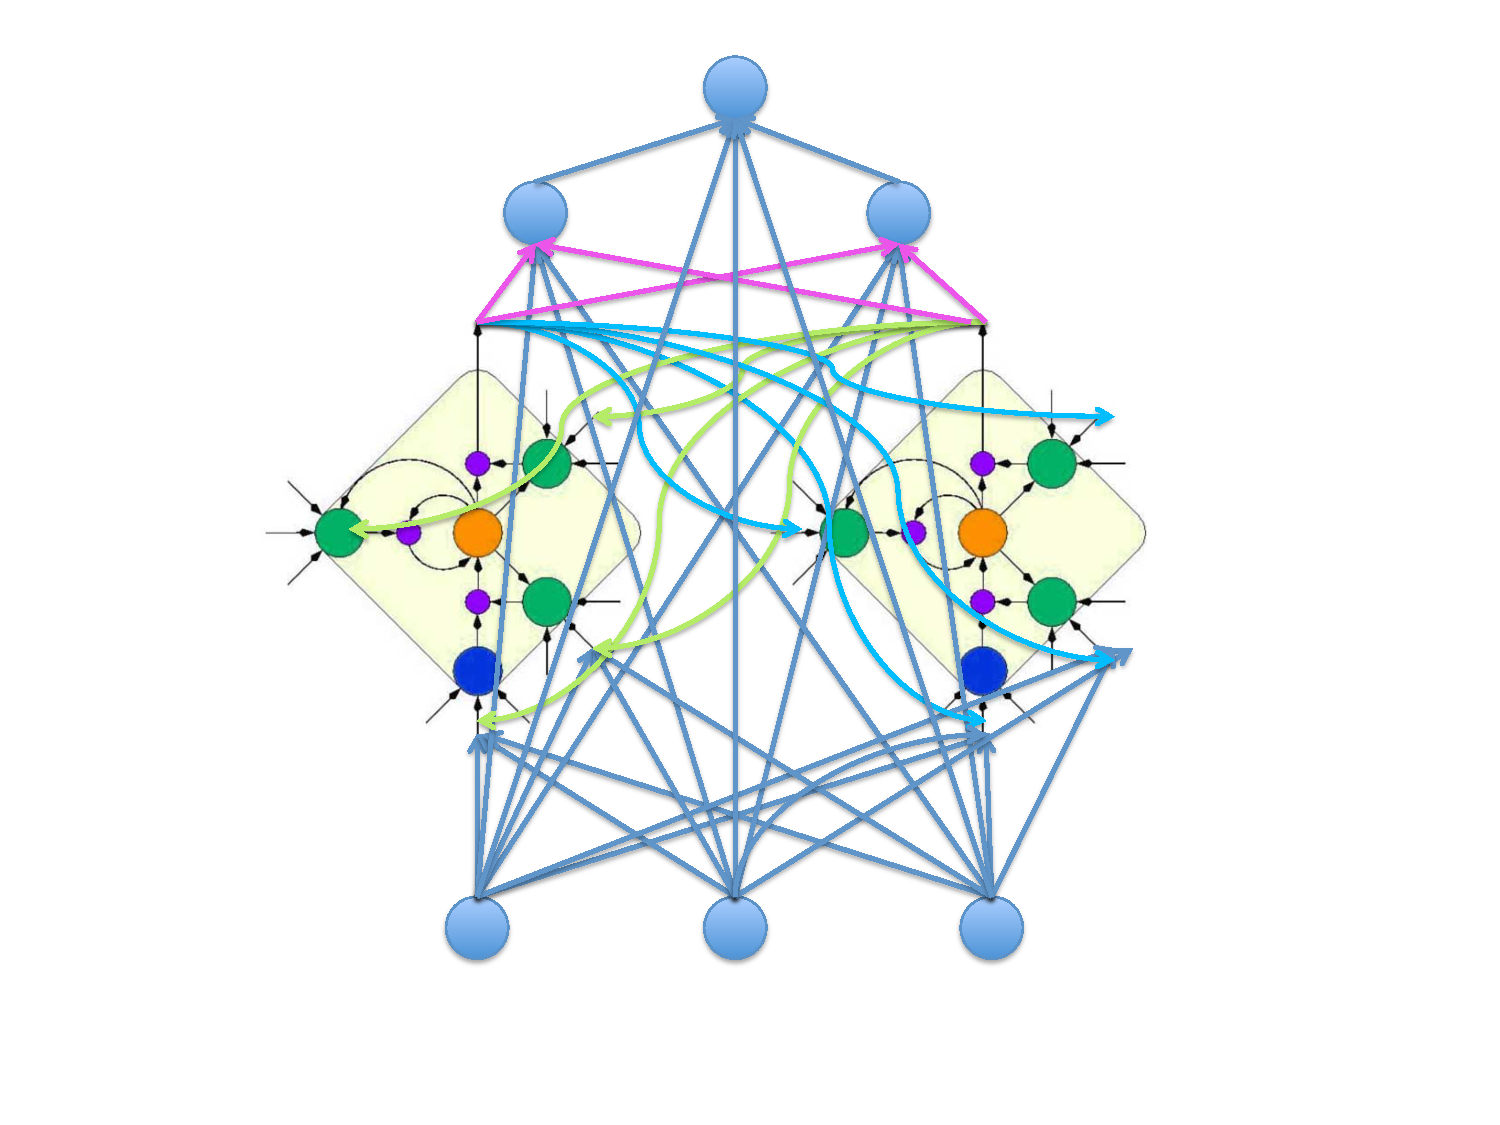
\includegraphics[scale = 0.5]{Pictures/LSTM/lstm_mixture_model.pdf}\\
  \caption{LSTM混合模型}\label{Fig:lstm_mixture}
\end{figure}



\section{LSTMP300Net}

在这一节中, 我们利用LSTM进行P300分类。 如第三章数据集介绍, 这里我们应用同样的P300波形进行P300检测。 由于P300信号为采集的时序信号, 所以采用时序模型更为合适。 





\chapter{总结}

本文

%\chapter{其他一些使用技巧}

如果在生成文档时发生错误,不要惊慌,可以先把生成的文件全部删除再试一次。
就是把除了tex文件外的其它同名文件都删掉。

使用WinEdt编辑tex文件时,如果嫌命令太长打着费劲,试试只输前几个字母然后按
“Ctrl+Enter”键,哈!WinEdt替你把剩下的部分补全了。

遇到问题不要慌,看下方小窗口里提示的出错信息,会有很多提示你错在哪里的。

不同系统下生成的eps可能会有兼容问题,
如本模版中的setroot.eps和rffndb.eps,在xp和windows 7 x64似乎不能通用。
解决方案很简单,
只要用bmeps -p 1 -c setroot.jpg setrooteps重新生成一次即可解决。
rffndb.eps生成命令同setroot.eps。

这个文档我用的是gVim编辑的,gVim自带的自动补全功能比WinEdt更强大,让我在
编写这个文档时省了不少重复工作量。

如果会使用make程序,那么使用Makefile来生成文档更方便一些。

在UTF-8版本中,如果一个命令后紧跟汉字,比如像这样“\verb+songti好的+”,
编译的时候就会报错,处理办法就是在命令后面加一个空格或者一个大括号,就像这样:
“\verb+songti 好的+”或者“\verb+songti{}好的+”

差不多了,就写这几条吧,想起来什么再写。

把另外几个参考文献当引用例子使用一下:专利\cite{WangZL},标准\cite{WangStd},
电子文档\cite{ZLB:1997},期刊文章\cite{LUOZ:2007},
学位论文\cite{wang:2008,wangmt:2008}。

这份文档从规划到完成,历时近20日,也是自己\LaTeX 学习一个总结吧。


\ZJUbackmatter
%%%%%%%%%%%%%%%%%%%%%%%%%%%%%%
%% 参考文献
%%%%%%%%%%%%%%%%%%%%%%%%%%%%%%
\ZJUthesisbib{thesisbib}

%%%%%%%%%%%%%%%%%%%%%%%%%%%%%%
%% 附录
%%%%%%%%%%%%%%%%%%%%%%%%%%%%%%
%\appendix
%\chapter{附录A - 贡献者}

\textbf{shuwei1204@163.com}:主要贡献者,原始项目地址: \\
http://code.google.com/p/zjuthesistex/downloads/list 

\textbf{ibillxia@gmail.com}:当前项目创建者,在原始项目上做了少许修改和扩充。

\chapter{附录B - 版本更新}
版本更新记录。



%%%%%%%%%%%%%%%%%%%%%%%%%%%%%%
%% 索引
%%%%%%%%%%%%%%%%%%%%%%%%%%%%%%
%\ZJUindex

%%%%%%%%%%%%%%%%%%%%%%%%%%%%%%
%% 个人简历
%%%%%%%%%%%%%%%%%%%%%%%%%%%%%%
%\begin{resume}
\begin{enumerate}
\item{第一条的内容}
\item{第二条内容}
\end{enumerate}
\end{resume}


%%%%%%%%%%%%%%%%%%%%%%%%%%%%%%
%% 发表论文目录
%%%%%%%%%%%%%%%%%%%%%%%%%%%%%%
%\begin{publications}
已发表学术论文:
\begin{enumerate}
\item{Rachel Zhang, Gang Pan, Yueming Wang, Zhenfang Hu. High-fidelity compression of extracellular recordings from motor cortex[C]. In Neural Networks (IJCNN), 2014 International Joint Conference on. IEEE,
2014, 3879–3886.}
\end{enumerate}

已投稿学术论文:
\begin{enumerate}
\item{Ruiqing Zhang, Zhenfang Hu, Yueming Wang, Gang Pan. High-fidelity compression of extracellular recordings from motor cortex[J]. In NeuralComputing. 状态:修改一次, minor revision.}
\end{enumerate}
\end{publications}


%%%%%%%%%%%%%%%%%%%%%%%%%%%%%%
%% 致谢页
%%%%%%%%%%%%%%%%%%%%%%%%%%%%%%
%\begin{thanks}
在我写这个文档的过程中,得到了网络上很多网贴的帮助,在此感谢baidu,Google,感谢
~CTeX 社区http://www.ctex.org,\LaTeX{}学习园地:http://blog.sina.com.cn/wangzhaoli11,
中科大~CTAN~镜像http://mirrors.ustc.edu.cn/CTAN/,水木社区\TeX{}版等网站、论坛,
其他一些较小的个人网站,论坛不再一一点名,在此一并感谢。
感谢浙江大学数学系提供的原始模版,感谢88\TeX{}版。
\end{thanks}


\end{document}
